\documentclass[12pt]{third-rep}

\newcommand{\uIP}{\mu{}IP}

%\includeonly{chapter1}

% Add draft header
\usepackage{fancyhdr}
\pagestyle{fancy}
\lhead{}  % left head
\chead{Draft: \today} % centre head
\lfoot{}
\cfoot{\thepage}
\rfoot{}

\usepackage{url}

\title{3D Printer ARM-Based Electronics Replacement}
\author{Jonathan Heathcote}
\supervisor{Alasdair Rawsthorne}
\reportyear{2012}

%% this defines the file that contains the text of the abstract, there
%% must be one of these by the time you submit your report.
\abstractfile{abstract.tex}

%% this defines the file that contains the acknowledgements (it can be
%% omitted if you don't feel like thanking anyone
\thanksfile{thanks.tex}

% Uncomment the following line if you want to change the name of the
% Bibliography to References
\renewcommand{\bibname}{References}

%%%%%%%%%%%%%%%%%%%%%%%%%%%%%%%%%%%%%%%%%%%%%%%%%%%%%%%%%%%%%%%%%%%%%%%%%%%%%%%%

\begin{document}
	% Front matter
	\dotitleandabstract
	
	\tableofcontents
	\listoffigures
	\listoftables
	
	% Chapters
	\chapter{Introduction}
	
	% TODO: Get rid of that trailing two line page...
	
	3D printing is a manufacturing process where computer models of objects are
	automatically reproduced in a physical form \cite{additivemanufacturing}.
	Figure \ref{fig:gearCube} shows an example of a complex 3D printed object.
	Various 3D printing technologies exist, some of which have gained a number of
	hobbyist-friendly implementations. In this project, a number of improvements
	the popular Makerbot Cupcake CNC 3D printer were made to improve its
	performance.
	
	\begin{figure}
		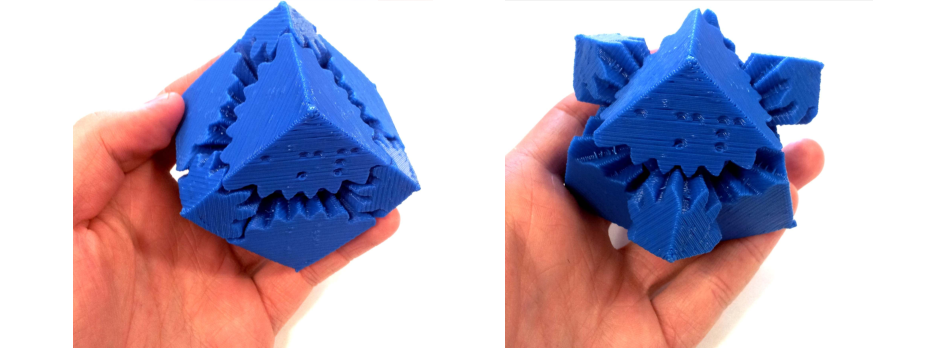
\includegraphics[width=1\textwidth]{diagrams/gearCube.pdf}
		\caption{3D printed `Gear Cube' produced by the printer upgraded in this
		project}
		\label{fig:gearCube}
	\end{figure}
	
	In this chapter the applications of 3D printing are examined followed by an
	introduction to the Makerbot and the improvements made by this project.
	
	\section{Applications}
		
		3D printing technologies allow complex objects, including complete
		mechanisms, to be easily manufactured based on digitized designs in one go
		with a single piece of equipment. Various materials are used including
		metal, various plastics, resins and even sugar \cite{candyfab}.
		
		Rapid prototyping is an obvious application where the flexibility to quickly
		manufacture a wide range of objects extremely valuable. For example, Boeing
		are using 3D printing to reduce the tooling cost and speed up prototyping
		its aeroplanes \cite{boeing3dprint}.
		
		Because there is no tooling cost associated with changing a design, custom
		manufacturing is also possible. This has applications both for personalised
		goods and more recently in the manufacture of bespoke medical implants
		\cite{jaw}.
		
		The cost of entry-level 3D printers has recently become much lower with DIY
		devices such as the RepRap costing between \$300 and \$620 to build
		\cite{costsdown,reprap}. This has helped grow communities such as
		Thingiverse where people share their designs for printable objects with the
		goal of making physical things as easily accessible as any other digital
		media \cite{thingiverse}.
	
	\section{Makerbot}
		
		\label{sec:makerbot_basics}
		
		The Makerbot (figure \ref{fig:makerbotOrig}) is an open source, DIY 3D
		printer which can produce plastic objects up to
		$10\cm\times10\cm\times13\cm$ in size.  It consists of a moving platform
		onto which an `extruder' melts plastic filament and deposits a thin strand
		of plastic (figure \ref{fig:printerBasics}). Objects are produced by moving
		the platform underneath the extruder and to form layers of plastic which are
		stacked one on top of each other until the complete shape is formed. Figure
		\ref{fig:slicing} shows how a cone (A) might be sliced into layers (B) and
		how each layer might be printed (C).
	
		\begin{figure}
			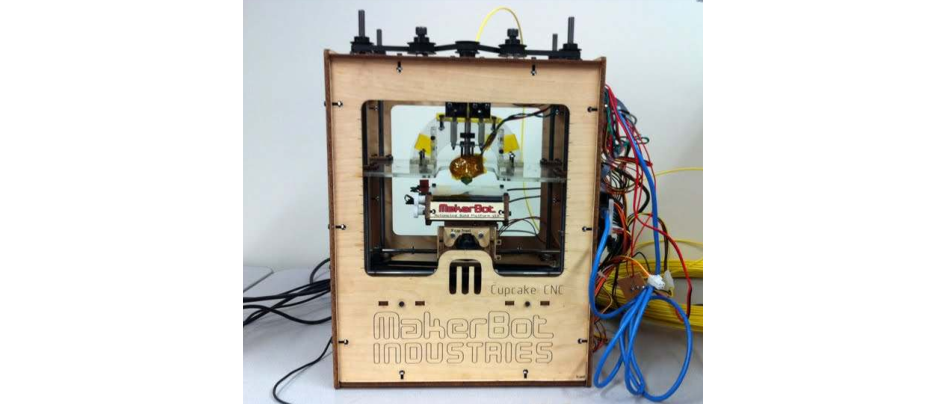
\includegraphics[width=1\textwidth]{diagrams/makerbotOrig.pdf}
			\caption{Unmodified Makerbot Cupcake CNC (photo by Rayshobby
			         \cite{rayshobby})}
			\label{fig:makerbotOrig}
		\end{figure}
	
		\begin{figure}
			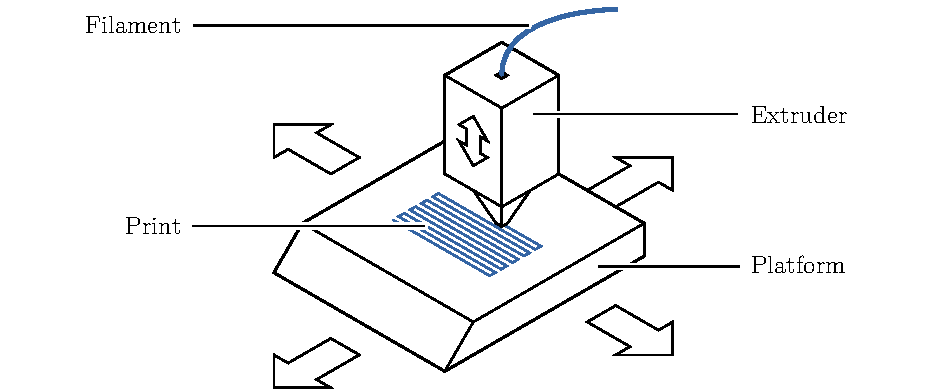
\includegraphics[width=1\textwidth]{diagrams/printerBasics.pdf}
			\caption{Makerbot key components}
			\label{fig:printerBasics}
		\end{figure}
		
		\begin{figure}
			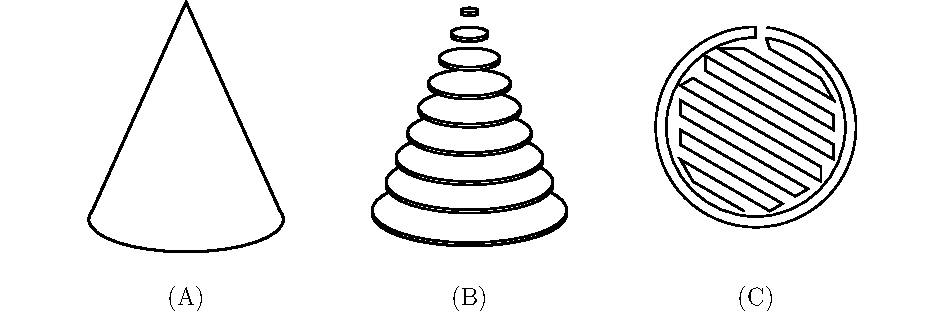
\includegraphics[width=1\textwidth]{diagrams/slicing.pdf}
			\caption{Slicing a 3D model into layers to be printed}
			\label{fig:slicing}
		\end{figure}
		
		Software running on a computer handles the process of slicing a 3D model and
		generating the list of movements required to print it out.  A simple
		microcontroller on the Makerbot receives this list of instructions and
		generates the carefully timed electronic signals needed to drive the
		printer's components.
		
	\section{Project Motivation and Goals}
		
		\label{sec:aims}
		
		The Makerbot, while a very capable machine, has many limitations in its
		hardware, electronics and firmware. In this project the control electronics
		and microcontroller are the primary area for improvement. The existing
		system has trouble with complex designs where dense sequences of
		instructions exceed the microcontroller's limited resources and slow serial
		interface. The electronics are also a complicated configuration of several
		circuit boards using clunky mechanical relays.  Finally, the printer does
		not have sensors to indicate the positions of the platform and extruder
		requiring the platform to be carefully positioned before prints. This is a
		time consuming and error prone task which also means that the printer can't
		detect mechanical errors during printing.
		
		In this project, each of these three complaints are addressed by the
		following primary project goals:
		\begin{description}
			
			\item[Simplify control electronics] Produce a single board which contains
			all required components using only reliable solid-state parts.
			
			\item[Improve performance] Upgrade to a more powerful microcontroller and
			develop new firmware to exploit the resulting improvements in speed and
			communications capabilities.
			
			\item[Add sensors for platform and extruder movements] End-stop sensors at
			the end of each axis of movement will be added to allow the system to
			position itself.
			
		\end{description}
	
	\section{Report Outline}
		
		This report first discusses the background of the project covering 3D
		printing and the technologies selected for the project. In chapter
		\ref{sec:design} the design of system is proposed followed by details of the
		implementation in chapter \ref{sec:implementation}. Chapter
		\ref{sec:testing} describes how the system was tested and evaluates the new
		system's performance. Finally, chapter \ref{sec:conclusions} concludes the
		report and describes opportunities for future work following on from the
		project.

	\chapter{Background}
	
	% TODO: Background Citations
	
	\label{sec:background}
	
	In this chapter the background of the project is described. The principle
	components of the Makerbot are discussed in more detail followed by a
	description of the tasks carried out by the firmware required to drives them.
	Afterwards, the ARM based `Mbed' microcontroller used in this project is
	introduced along with the `FreeRTOS' operating system.
	
	\section{Makerbot}
		
		The Makerbot Cupcake CNC used in this project is the first generation of a
		series of printers based on the RepRap 3D printer \cite{makerbotcupcake}.
		The RepRap, and consequently the Makerbot are open designs which are freely
		available for use and modification.
		
		In this section, the primary components of the printer are described
		followed by the electronics, firmware and microcontroller that drives them.
		
		\subsection{Printer Components}
			
			The printer can be broken down into three major components, the axes along
			which the machine's components can move, the extruder which melts the
			plastic and the platform itself on which the design forms. Each of these
			are described below.
			
			\subsubsection{Axes of Movement}
				
				% TODO: Diagram/pictures?
				
				There are three axes of movement in the Makerbot. Two horizontal axes
				along which the platform can travel, the X and Y, axes, and one vertical
				axis along which the extruder is moved, the Z axis.
				
				The X and Y axes move along rails and are belt driven by a stepper
				motor. The Z axis moves up and down four threaded rods which are
				connected together via a belt and driven by a single stepper motor. When
				the threaded rods turn, the extruder is moved by the screwing effect of
				the rods.
				
				Stepper motors allow precise movements to be made. In contrast with
				simple DC motors which turn electrical energy into continuous movement,
				stepper motors turn energy into discrete `steps' of movement.
				
				A simple stepper motor consists of four toothed electromagnets and a
				toothed magnetic central rotor. By turning on each electromagnet in
				sequence, the teeth of the rotor are moved to align with the energised
				electromagnet causing a single step of movement to be executed (an
				example is given in figure \ref{fig:stepperMotor}) \cite{steppers101}.
				
				\begin{figure}
					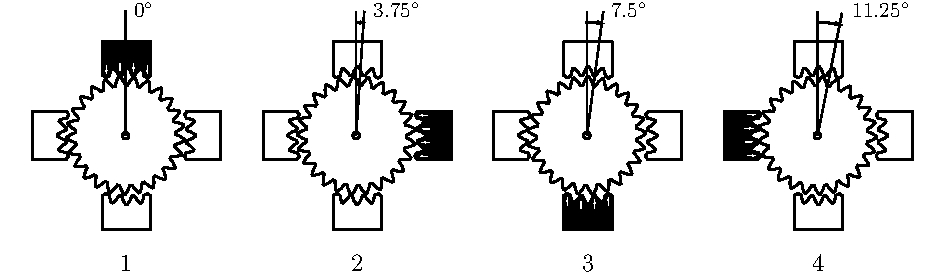
\includegraphics[width=1\textwidth]{diagrams/stepperMotor.pdf}
					\caption{Stepper motor operation}
					\label{fig:stepperMotor}
				\end{figure}
				
				By controlling these steps, the motor's rotation and speed can be
				exactly controlled. Stepper motors lack active feedback mechanisms and
				rely solely on the motor successfully completing every step. This
				assumption does not hold if the motor is unable to provide enough torque
				(turning power) to move its load. As a result, the motors used by the
				printer are designed to be powerful enough to reliably provide the
				torque needed so that sensors are not needed to judge the position of
				the system.
				
			\subsubsection{Extruder}
				
				The extruder uses a simple DC motor and gearbox to force a filament of
				acrylonitrile butadiene styrene (ABS) plastic, the material Lego is made
				from, into a heater and out of a fine nozzle (figure \ref{fig:extruder}).
				A temperature sensor is installed in the heater allowing the temperature
				to be carefully controlled to ensure an even flow.
				
				\begin{figure}
					
\includegraphics[width=1\textwidth]{diagrams/extruder.pdf}
					\caption{Extruder components}
					\label{fig:extruder}
				\end{figure}
				
			\subsubsection{Platform}
				
				The platform contains a heated build surface which  helps prevent prints
				warping and this also improves the adhesion of the print to the build surface.
				
				The build surface is also a conveyor belt powered by a small DC motor
				and gearbox. It is used to eject printed objects after printing
				completes allowing continuous printing operations.
				
		\subsection{Electronics}
		
			The Makerbot is controlled by the RepRap's generation 3 electronics
			\cite{reprapelectronics}. These
			consist of:
			\begin{description}
				
				\item[Motherboard] This circuit board hosts an 8-bit microcontroller
				which communicates with a computer via a custom serial interface and
				controls the printer's operation.
				
				\item[Extruder Controller] This circuit board hosts a second small
				microcontroller along with electronics for the extruder's motor and
				temperature sensor.  The extruder controller communicates with the
				motherboard via a custom RS485 interface.
				
				\item[Relay Board] This circuit board contains a mechanical relay for
				turning each of the two heaters on and off. The relay board is driven by
				the extruder controller using simple digital signals.
				
				\item[Stepper Motor Driver ($\times 3$)] Circuit boards which produce
				the high-power signals required to drive the stepper motors. These
				boards are connected to the motherboard via a simple digital interface
				that abstracts away many of the electrical and timing difficulties
				driving a stepper motor.
				
			\end{description}
	
		\subsection{Microcontrollers}
			
			The electronics use a pair of Arduino-compatible microcontrollers to drive
			the printer. These devices have a fairly minimal 8-bit instruction set,
			limited amounts of memory (4KB of RAM) and a very limited set of options
			for high-speed communications. A faster microcontroller capable of faster
			communication and command processing is needed to solve the performance
			problems described in \S\ref{sec:aims}.
		
		\subsection{Firmware}
			
			The firmware on the microcontrollers is responsible for two main tasks:
			receiving print data from a computer and producing the signals required
			for printing. The signals produced have strict `real-time' timing
			requirements and so to meet these, specialised timing hardware within the
			microcontroller must be used.
			
			3D printers typically receive print data in the form of G-code files
			\cite{reprapgcode}. G-code is the de facto standard for controlling
			computer numerical control (CNC) machines such as 3D printers, laser
			cutters and lathes. The language is human readable and defines
			step-by-step instructions for machine actions such as `move to (X,Y,Z)' or
			`enable heater'.
			
			The RepRap generation 3 firmware on the motherboard uses a custom serial
			protocol to communicate with the host computer. This protocol is designed
			to be simple for the microcontroller to use and, as well as various
			diagnostic features contains a compressed version of G-code.
		
		\subsection{Support Software}
			
			The G-code used by the printer is generated from 3D models using an
			open-source tool called Skeinforge \cite{skeinforge}. Skeinforge is
			typically used as part of ReplicatorG, a graphical user interface for
			preparing and printing 3D models \cite{replicatorg}. ReplicatorG can also
			handle the translation of G-code into the compressed format used by the
			RepRap firmware.  Other less mature tools, such as Slic3r, are available
			but less frequently used.
		
	\section{ARM \& Mbed}
		
		As well as high-performance processors designed for phones, ARM also design
		the Cortex-M series of microcontrollers. For this project a Cortex-M3 based
		`Mbed' microcontroller was chosen to replace the pair of existing 8-bit
		microcontrollers \cite{mbed}. The reasons for the suitability of this choice
		are justified in this section.
		
		\subsection{Mbed}
			
			The Mbed is a small microcontroller prototyping board centred around the
			NXP LPC1768, ARM Cortex-M3 based microcontroller (figure \ref{fig:mbed}).
			It has has four debugging LEDs, a USB port for loading programs various
			input/output facilities including facilities for attaching an Ethernet
			port. The pins on the device expose these input and output capabilities
			and fit into standard 0.1" spaced circuit boards and prototyping
			breadboards.
			
			\begin{figure}
				
\includegraphics[width=1\textwidth]{diagrams/mbed.pdf}
				\caption{Mbed microcontroller}
				\label{fig:mbed}
			\end{figure}
			
			The Mbed provides a USB flash drive-like interface. This interface is used
			to program the device by simply copying a binary file onto it. This
			mechanism is used to support the device's unusual choice of purely
			web-based official development tools. Web-based development was not ideal
			for this project and an alternative solution is discussed in
			\S\ref{sec:compiler} allowing conventional development tools to be used.
		
		\subsection{NXP LPC1768}
			
			The LPC1768 microcontroller behind the Mbed provides the ARM Cortex-M3
			processor with various useful peripherals. It runs at up to $100\MHz$ and
			has $32\KB$ of ram \cite{lpc1768}.  While still a seemingly tiny amount
			compared to even a modest smart phone, this is a large amount for a
			microcontroller without the overhead of running a fully-fledged general
			purpose operating system and associated software.
			
			The chip contains various peripherals such as hardware timers, analog
			interfaces and, importantly, fast Ethernet support. These timers will, as
			with the previous microcontrollers, be vital for driving the electronics
			properly. Analog inputs are also needed to interface with the electronics.
			Ethernet support will allow the microcontroller to quickly receive
			detailed print data over the network.
			
			As well as these features, ARM devices are widely used and boast mature,
			open-source development tools making it an ideal choice for expanding the
			open-source Makerbot design.
			
	\section{Real-Time Operating Systems}
		
		The firmware consists of various complimentary parts (such as communication
		and control), which are easily managed with the use of an operating system.
		Due to the absolute timing and performance requirements FreeRTOS, a
		real-time operating system (RTOS), was selected.
		
		\subsection{Differences With Non-Real-Time Systems}
			
			Real-time operating systems, like other operating systems, provides a
			scheduler which allows multiple processes to run as if simultaneously. It
			also provides facilities for communicating between these processes. Unlike
			regular operating systems, an RTOS can provide exact timing guarantees.
			They are also generally be targeted at microcontroller development with
			tight resource constraints and without the need for extra hardware such as
			a memory management unit (MMU).
			
		\subsection{FreeRTOS}
			
			FreeRTOS is a widely used, open-source RTOS designed for use with a range
			of microcontrollers, including many Cortex-M3 based devices
			\cite{freertos}. The two key features provided by FreeRTOS are `tasks' and
			`queues' which are described below.
			
			\subsubsection{Tasks}
				
				A system built on FreeRTOS can be structured as several tasks
				executing in parallel. Tasks are similar to processes or threads on a
				conventional operating system with each task having its own set of
				registers and a stack.
				
				Because the microcontroller can only run one task at once, the FreeRTOS
				uses preemptive scheduling to approximate this behaviour where the
				current task is periodically interrupted by a timer (preempted) and a
				different task put in its place. If tasks are switched fast enough, they
				appear to run simultaneously.
				
				Tasks may be given different priorities and can be suspended until
				events such as a timer expiring or a hardware resource becoming
				available occur. The timing of the operating system's actions can be
				guaranteed allowing real-time systems to be developed.
				
			\subsubsection{Queues \& Mutexes}
				
				To provide synchronisation and communication between tasks, FreeRTOS
				provides a queue structure. Queues are defined which allow data to be
				inserted or removed with a first-in-first-out (FIFO) access scheme.
				
				These queues can be used safely by multiple tasks simultaneously without
				race conditions and so are ideal for inter-task communication.  Because
				of this safety, they also form the basis for standard parallel
				programming constructions such as semaphores and mutexes.
				
				When accessing a FreeRTOS queue a task may become blocked, for example,
				when adding an item to a queue that is already full. FreeRTOS can
				provide timing guarantees on timeouts waiting for these functions to
				complete. It also allows a task's priority to be temporarily raised when
				resumed after a blocking call, ensuring it is scheduled as soon as
				possible, reducing the delay before any new data data is processed.

	\chapter{Design}
	
	\label{sec:design}
	
	% TODO: Past tenseify!
	
	In this chapter a system design is proposed based on the considerations of the
	previous chapter. An overview is given which is followed by a more detailed
	description of the important components of the system.
	
	% TODO: Requirements
	
	\section{Overview}
		
		The 3D Printing system can be divided up into three main parts. First is the
		computer software used to design the object to be printed and to generate
		the G-code instructions which will cause the object to be printed. The
		second is microcontroller firmware which processes the G-code and drives the
		printer electronics appropriately. Finally, there is the actual printer
		hardware consisting of electronics driving the various motors, heaters and
		sensors.
		
		% TODO: Remove detail (diagram out of date anyway)
		\begin{figure}[here]
			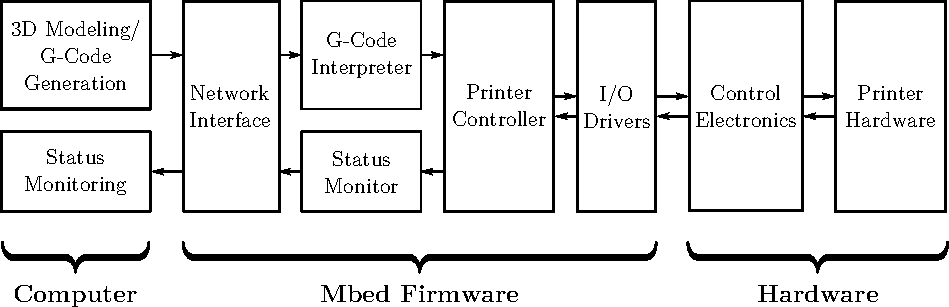
\includegraphics[width=1\textwidth]{diagrams/systemDiagramTop.pdf}
			\caption{High-level diagram of overall system architecture.}
			\label{fig:systemDiagramTop}
		\end{figure}
	
	\section{Computer Software}
		
		This project is principally focused on the development of the firmware and
		electronics used by the printer. The process of generating 3D models and
		G-code is out of the scope of this project and will be carried out using
		off-the-shelf, open source tools.
		
		A limited amount of software will be provided which will allow G-code to be
		streamed to the printer and for the printer's status to be fetched.
	
	\section{Firmware}
		
		The microcontroller firmware will consist of three main components running
		on top of the FreeRTOS operating system (see Figure
		\ref{fig:systemDiagramFirmware}). The first will be the \uIP{} network stack
		for communication with the computer software. The second, is a G-code
		processing pipeline which will translate G-code into an appropriate sequence
		of commands to the electronics. The third component is a driver interface
		for the required components of the Mbed will be needed.
		
		\begin{figure}[here]
			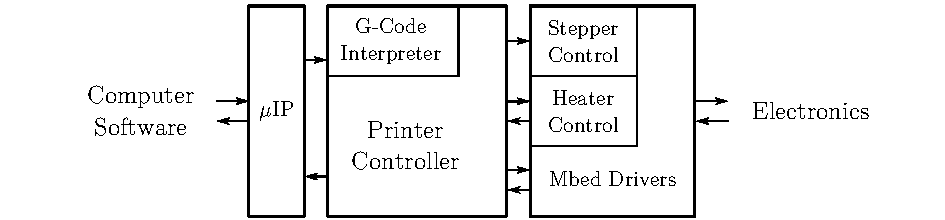
\includegraphics[width=1\textwidth]{diagrams/systemDiagramFirmware.pdf}
			\caption{Major components of the Mbed firmware}
			\label{fig:systemDiagramFirmware}
		\end{figure}
		
		\subsection{Network Interface}
			
			The firmware will provide an interface for sending G-code and an interface
			for querying the printer's status.
			
			The G-code interface should be a simple open port which silently accepts
			and G-code streams and feeds them into the pipeline. It will need to
			support flow control as the rate at which the printer is able to accept
			G-code instructions will vary depending on what instructions are being
			executed. For example while waiting for heaters to warm up no instructions
			will be executed but during complex movements, many instructions may be
			executed in rapid secession. The interface must also be reliable. A
			missed, corrupted or out-of-order G-code instruction would cause
			unexpected results.
			
			TCP offers both reliable communication and flow control mechanisms and is
			implemented in \uIP{}.\footnote{Some G-code implementations have error
			checking and retransmission mechanisms but these are clunky and designed
			for use with serial connections.} Unfortunately,
			the TCP flow-control implementation in \uIP{} was found to be buggy. Due
			to time constraints and the compact nature of \uIP{} a minimal custom
			UDP-based protocol should be used as a work-around.
			
			% XXX: Really mention UDP hack here?
			
			The status querying interface has few requirements and should be kept
			minimal to save microcontroller and development resources. A
			\verb+telnet+ compatible interface (which is both human and machine
			readable) should serve this purpose.
		
		\subsection{G-code Processing Pipeline}
			
			The main task of the firmware is to process incoming G-code from the
			network and to control the printer appropriately without stalling. A
			pipeline architecture (Figure \ref{fig:firmwarePipeline} was selected
			where G-code is buffered before being interpreted and converted into
			lower-level commands. The low-level commands are placed in a buffer and
			then executed in sequence to drive the printer.
			
			\begin{figure}[here]
				
\includegraphics[width=1\textwidth]{diagrams/firmwarePipeline.pdf}
				\caption{G-code processing pipeline}
				\label{fig:firmwarePipeline}
			\end{figure}
			
			In order to reduce stalls due to data processing between commands the
			low-level commands used at the end of the pipeline exchange space for
			computation time by keeping all command arguments in formats directly used
			by the printer (e.g. distances in an integral number of steps and not
			floating point values in millimetres).
			
			Nearer the start of the pipeline, we want to minimise the effect of
			network latency by having a large buffer which gives the network time to
			respond to changes in the rate of command execution.
			
			Finally, by assigning a high priority to the Printer Controller we can
			minimise the latency between a command completing and another starting,
			especially during very short bursts of extremely detailed movements.
		
		\subsection{G-code Interpreter}
			
			Though existing G-code interpreters are available they are generally
			tightly integrated with directly controling the electronics and not easily
			used standalone. G-code implementations also vary widely with 3D printers
			generally only using a very small subset of the available features. As a
			result, a small G-code interpreter will be implemented for the required
			subset of G-code.
		
		\subsection{Drivers}
			
			In order to interface with the electronics and facilitate accurate timing
			various peripherals on the Mbed will require supporting driver code. In
			particular, the following features will be needed:
			
			\begin{description}
				\item[General-Purpose Input/Output (GPIO)]
					Allows TTL (Transistor-Transfer-Level) digital signals to be produced
					or read from the pins on the microcontroller. For example stepper
					control signals, end-stop signals.
				
				\item[Analog Input]
					Read analog signals from the electronics. For example readings from
					temperature sensors.
				
				\item[Timer]
					Produce interrupts at precisely timed intervals to allow stepper
					control signals to be produced.
				
				\item[Watch-dog Timer]
					To ensure fail-safe behaviour, a watch-dog timer can be used to reset
					and power down the system in the event of software malfunction.
			\end{description}
	
	
	\section{Electronics \& Hardware}
		
		Most of the work of this project will be focused on the electronics used to
		drive the printer's hardware rather than the hardware itself though some
		new sensors will be added.
		
		\subsection{Stepper Control}
			
			The printer's three primary axes are controlled by stepper motors which require
			complex circuitry to drive. The previous electronics used off-the-shelf RepRap
			stepper motor drivers \cite{stepperMotorDriver23}. Each of these boards
			connects directly to the stepper motor coils, an ATX power supply and a
			TTL control interface. They also provide a connection for two end-stop
			sensors to be attached (the output from which they passively forward back
			through the TTL connection).
			
			\begin{figure}[here]
				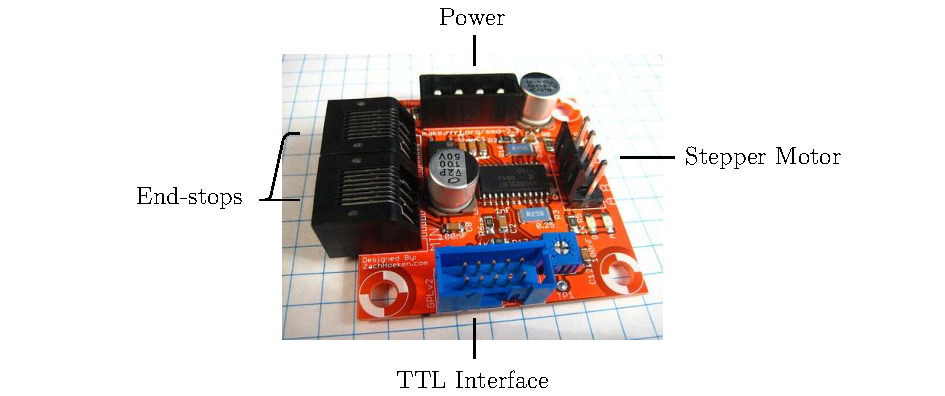
\includegraphics[width=1\textwidth]{diagrams/stepperControllerBoard.pdf}
				\caption{Stepper controller board with connections labelled. (Photo \cite{stepperControllerBoardPhoto})}
				\label{fig:stepperControllerBoard}
			\end{figure}
			
			These boards provide an enable, direction and step signal which allow
			the microcontroller to drive the steppers using three GPIO pins per axis.
		
		\subsection{Heater \& DC Motor Control}
			
			The heaters and motors both require large amounts of current at 12 volts
			to run. This far exceeds the output of the GPIO pins on the Mbed so a
			circuit will be needed to switch the power for these devices.
			
			Previously, mechanical relays were used to control the heaters but instead
			a solid-state solution should be sought to allow the posibility of varying
			heater power.
		
		\subsection{End-stops}
			
			By adding end-stop sensors on each axis, the axes can be accurately and
			consistently positioned at the start of a print job. Electronics
			compatible with the interface exposed by the stepper controller board will
			be required.
			
			Optical end-stops have been selected as the Makerbot has mounting holes at
			the end of each axis for mounting them.  Optical end-stops are also
			non-contact and so do not disrupt the movement of the axes.
			

	\chapter{Implementation}
	
	This chapter describes the implementation of the system in detail. First the
	electronics are described and followed by an explanation of the firmware.
	Finally, safety considerations and a brief discussion of the methods used is
	presented.
	
	
	\section{Electronics}
		
		% TODO: Some intro
		
		Two boards were produced, one which hosts the Mbed and the electronics
		needed to drive the heaters, motors and temperature sensors and another
		which provides an interface between the end-stops and stepper controller
		boards. The system as installed in the printer is shown in figure
		\ref{fig:electronicsPhoto} with the major components labelled.
		
		% TODO: Picture of up-to-date electronics
		\begin{figure}
			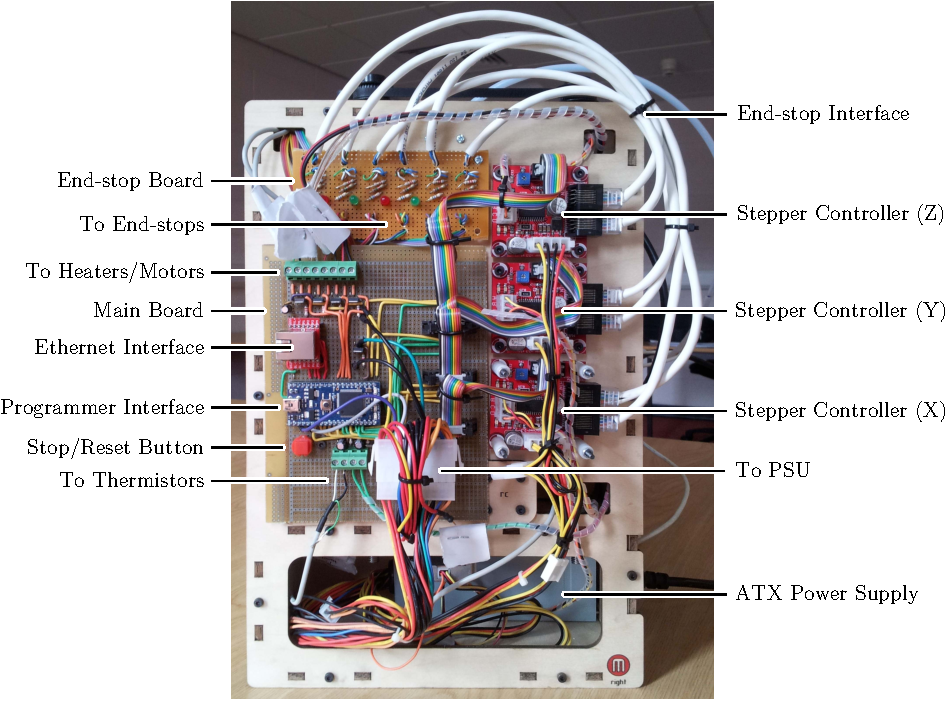
\includegraphics[width=1\textwidth]{diagrams/electronicsPhoto.pdf}
			\caption{Electronics installed with major connections labelled}
			\label{fig:electronicsPhoto}
		\end{figure}
		
		To keep the system simple to build using readily available tools, 0.1"
		spaced electronics were used throughout. These are easy to work with using
		only a standard soldering iron and basic tools. Components of this size can
		also be used in prototypes built on a solderless breadboard.
		
		The main board will host the Mbed, electronics for controlling the heaters,
		reading from the temperature sensors and connecting to the stepper
		controller boards. A second board is used for the end-stop electronics as
		these parts may be replaced separately from the main electronics and connect
		via the stepper controller boards.
		
		\subsection{Layout \& Board}
			
			A prototyping board designed for working with DIP (Dual In-line Package)
			components such as the Mbed was selected (Figure \ref{fig:dipBoard} B).
			Conventional strip board (\ref{fig:dipBoard} A) would require many
			connections to be cut between the two columns of pins of the device. The
			particular design chosen also includes a ready-made ground-plane.
			
			\begin{figure}
				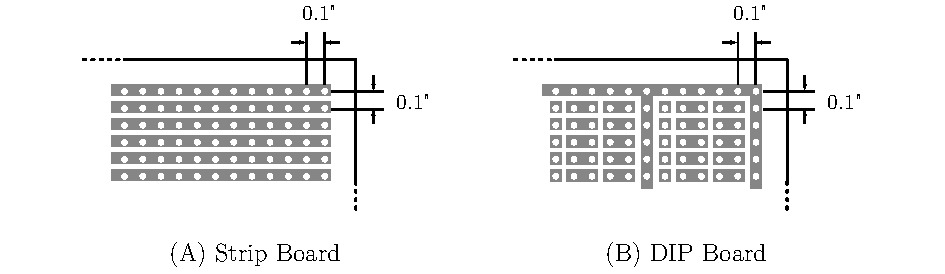
\includegraphics[width=1\textwidth]{diagrams/dipBoard.pdf}
				\caption{Types of prototyping board}
				\label{fig:dipBoard}
			\end{figure}
			
			\begin{figure}
				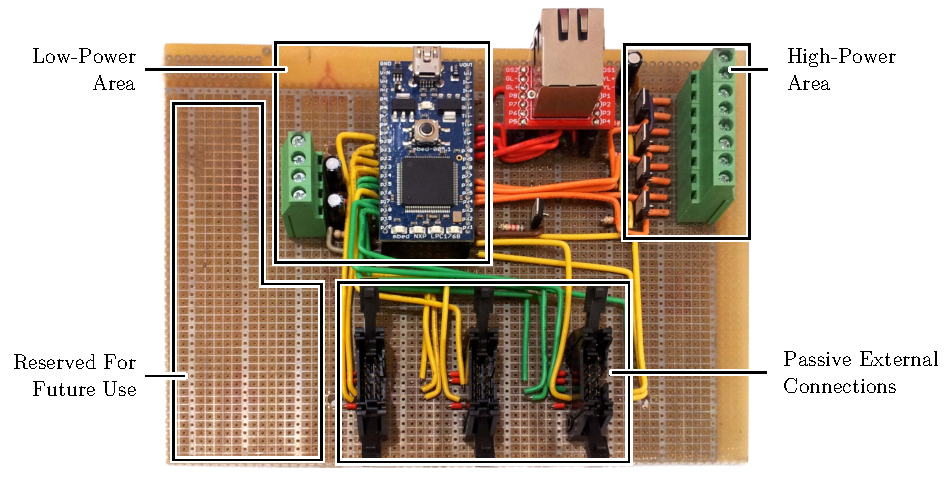
\includegraphics[width=1\textwidth]{diagrams/mainBoard.pdf}
				\caption{Top-level layout of main board (reset button and power
				         connections not shown)}
				\label{fig:mainBoard}
			\end{figure}
			
			The main board contains electronics for both low-power systems such as
			the Mbed and high-power systems such as the heater and motors and
			interference between these parts must be minimised. The high and lower
			power parts have been kept physically separate on the board (Figure
			\ref{fig:mainBoard}), each with their own power supply. The board also
			has a ground plane covering the whole board which also helps reduce
			noise\cite{pcb_design_notes}.
			
			A full circuit schematic and pin-out is given in Appendix
			\ref{sec:mainboardDiagrams}.
		
		\subsection{Heaters \& DC Motors}
			
			\label{sec:heatersAndMotors}
			
			% TODO: Part numbers, specs and fact check!
			
			The heaters and DC motors in the extruder and platform operate at a
			higher voltage and are considerably higher-current than the
			microcontroller can produce on its output pins. To control these a
			transistor is required.  An IRLU8729PbF MOSFET (Metal Oxide Field Effect
			Transistor) was selected as it can switch large loads up to 58A with
			very little on-resistance (reducing energy wastage through
			heat)\cite{MOSFET}.
			
			% TODO: Photo of MOSFET
			\begin{figure}
				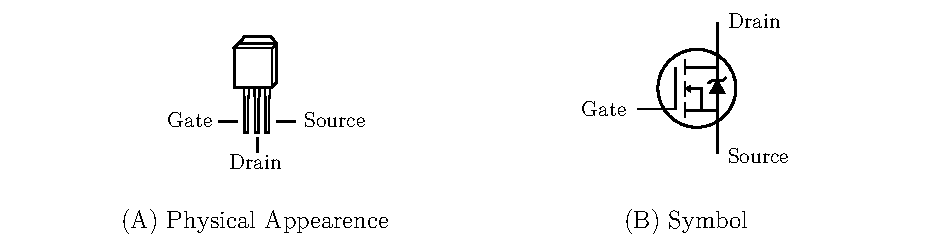
\includegraphics[width=1\textwidth]{diagrams/mosfetDiagram.pdf}
				\caption{Metal Oxide Semiconductor Field Effect Transistor (MOSFET)}
				\label{fig:mosfetDiagram}
			\end{figure}
			
			The MOSFET has three connections called the gate, drain and source
			(Figure \ref{fig:mosfetDiagram}). When the voltage between the gate and
			the source is 0V, no current flows from the drain to the source. As the
			voltage between the gate and drain are increased, the current allowed to
			flow increases rapidly when it passes a certain threshold (Figure
			\ref{fig:mosfetPerformance}). By connecting the gate to a pin on the
			Mbed and the source to ground, a large current from a device such as a
			heater or motor can be switched by connecting it through the drain to
			ground.
			
			\begin{figure}
				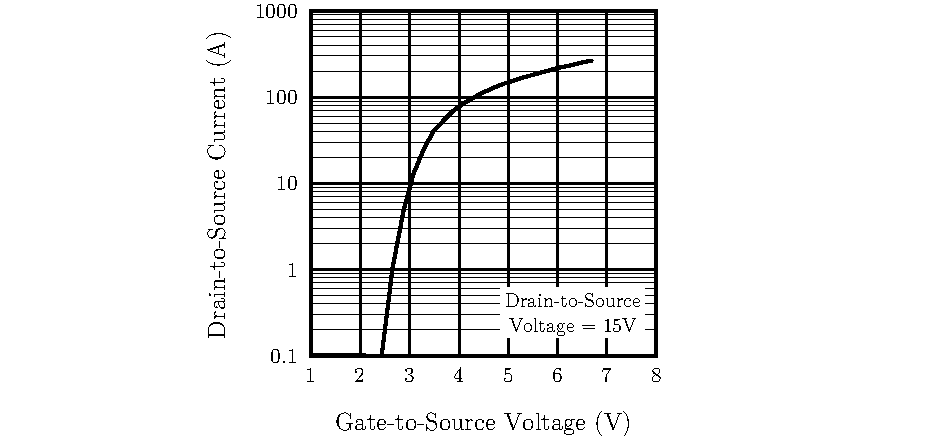
\includegraphics[width=1\textwidth]{diagrams/mosfetPerformance.pdf}
				\caption{IRLU8729PbF Typical Transfer Characteristics (reproduced from
				`Fig 3', \cite{MOSFET})}
				\label{fig:mosfetPerformance}
			\end{figure}
			
			The behaviour of a MOSFET when the gate is left floating (disconnected)
			is generally undefined and can damage the component. When the Mbed
			powers on its output pins default to a floating state which could cause
			a MOSFET to unexpectedly turn on or become damaged. To prevent this
			happening the gate is connected to ground via a pull-down resistor. When
			the output pin is floating the gate is pulled to 0V by the pull-down
			resistor. When the output of the pin is not floating, the gate is pulled
			to that voltage overriding the pull-down resistor. A high resistance
			value is used so that the Mbed can easily override the pull-down
			resistor.
			
			Figure \ref{fig:mosfetUsage} shows the circuit used to control the two
			heaters and two motors using a MOSFET and pull-down resistor.
			
			\begin{figure}
				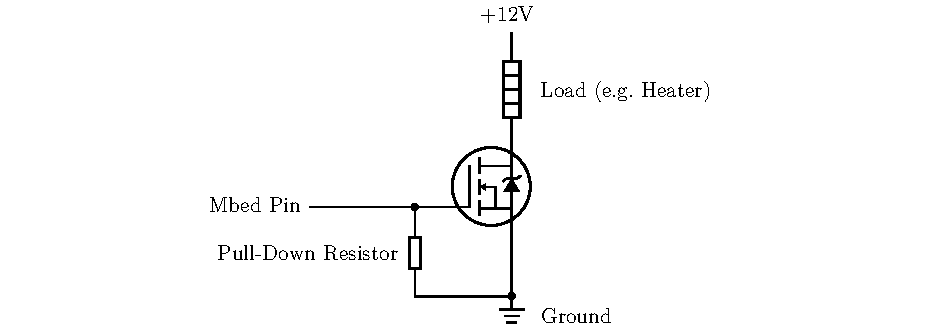
\includegraphics[width=1\textwidth]{diagrams/mosfetUsage.pdf}
				\caption{Example MOSFET circuit with pull-down resistor}
				\label{fig:mosfetUsage}
			\end{figure}
			
			When driving motors a `flyback diode' is usually used to prevent a
			voltage spike occurring when the power is removed from the motor. This
			voltage spike is caused by the magnetic field in the motor's coils
			collapsing. This is not included in the circuit as the MOSFETs used
			already contain an appropriate diode.
			
			It should be noted that this circuit does not allow the motors to be
			driven in both directions as this is not needed by the printer. If this
			was required, a more complex circuit (such as a H bridge) would be
			needed.
		
		\subsection{Thermistors}
			
			\label{sec:thermistor}
			
			To measure the temperature of the heaters, thermistors are used. The
			resistance of a thermistor changes non-linearly with temperature and is
			modelled using an equation derived from the Steinhart-Hart
			Equation\cite{Steinhart1968497}:
			\begin{equation}
				\frac{1}{T} = \frac{1}{T_0} + \frac{1}{\beta} \ln \left( \frac{R}{R_0} \right)
				\label{equ:steinhart}
			\end{equation}
			Where $T$ and $R$ are the current temperature and resistance of the
			thermistor, $T_0$ and $R_0$ are the temperature and resistance at a
			reference temperature and $\beta$ is a characteristic constant for the
			device available in the data-sheet.
			
			% TODO: Cite potential divider
			
			Using the Analog-to-Digital converter in the Mbed, voltages, but not
			resistances, can be read directly. A potential divider (Figure
			\ref{fig:potentialDiv}) is used to measure the resistance.
			\begin{figure}
				
\includegraphics[width=1\textwidth]{diagrams/potentialDiv.pdf}
				\caption{Potential divider}
				\label{fig:potentialDiv}
			\end{figure}
			A reference voltage $V_\textrm{ref}$ is placed across two resistors,
			$R_1$ and $R_2$, and the voltage between them at $V$ is measured. The
			relationship between these variables is
			\begin{equation}
				V = V_\textrm{ref} \frac{R_2}{R_1 + R_2}
			\end{equation}
			Thus, if the thermistor is placed as $R_2$, the resistance can be
			calculated using
			\begin{equation}
				R_2 = V_\textrm{ref} \frac{R_1}{V - V_\textrm{ref}}
				\label{equ:potdiv}
			\end{equation}
			
			% TODO: Resistor choice, specify thermistor
			
			The value of $R_1$ was chosen...
			
			Using (\ref{equ:steinhart}) and (\ref{equ:potdiv}) with a potential
			divider circuit will allow the temperature of the thermistor to be
			measured.
			
		
		\subsection{Stepper Motors}
			
			The stepper controllers chosen accept TTL signals and connect via a
			ten-pin insulation displacement connector (IDC). An IDC socket was
			placed on the board and the pins connected directly to the Mbed and
			ground plane as required. The pin-out for these connections is given in
			Appendix \ref{sec:stepperControllerPinout}.
			
			% TODO: IDC Picture
		
		\subsection{End-stops}
			
			Optical end-stops consist of a photo-interrupter containing an infra-red
			LED and a photo-transistor arranged across a gap (Figure
			\ref{fig:endstop}). Photons from the LED activate the photo-transistor
			allowing current to flow but when the gap is blocked, the transistor is
			switched off and no current flows.
			
			\begin{figure}
				
\includegraphics[width=1\textwidth]{diagrams/endstop.pdf}
				\caption{Photo-interrupter with a photo-transistor in a Darlington pair}
				\label{fig:endstop}
			\end{figure}
			
			Due to problems sourcing the interface boards for the end-stops, a
			circuit was built which is compatible with the stepper-controller
			interface for end-stops. $+5V$ and ground are provided and a TTL logic
			signal is expected by the interface. To ease debugging, an indicator LED
			is also provided which is lit when the end-stop is unobstructed.
			
			% XXX: Is it a pulldown?
			
			The LED in the photo-interrupter is driven via a current-limiting
			resistor and the signal output and indicator LED are connected through
			the photo-transistor. A pull-down resistor is used to pull the signal
			to ground when the photo-transistor is powered off.
			
			The circuitry is placed on a board with cables running to each end-stop
			(photo-interrupter) and to each of the CAT-5 sockets on the stepper
			controller boards. Strain-relief is included so that the connections are
			not damaged if the cables are caught in the machine. A circuit diagram
			is provided in Appendix \ref{sec:stepperControllerPinout}.
			
			% TODO: Picture of mounted endstop and board
			
			% XXX: Include resistor values and theory of operation?
			
			
		\subsection{Power}
			
			The printer uses an ATX power supply unit (PSU) commonly found in
			desktop computers. A 20-pin connector containing both power and various
			control signals for the power supply is used to power the main board
			(see table \ref{tab:atxConnectors}).
			
			\begin{table}[here]
				\centering
				\begin{tabular}{l l l}
					\toprule
					Signal & Colour & Notes\\
					\midrule
					Ground & Black  & \\
					+3.3V  & Orange & $\pm5\%$  Tolerance (Unused) \\
					+5V    & Red    & $\pm5\%$  Tolerance \\
					+12V   & Yellow & $\pm5\%$  Tolerance \\
					-12V   & Blue   & $\pm10\%$ Tolerance (Unused) \\
					\addlinespace
					Power Good  & Gray   & Signal asserted when all voltages are correct
					                       and stable \\
					+5V Standby & Purple & Power available at all times (Max 2A) \\
					+3.3V Sense & Brown  & Unused \\
					Power On    & Green  & Active-Low signal pulled up to +5V \\
					
					\bottomrule
				\end{tabular}
				
				\caption{20-pin ATX Connector Signals\cite{ATX}}
				\label{tab:atxConnectors}
			\end{table}
			
			The Mbed is connected to the 5V standby supply allowing it to remain
			booted and power on the system on demand. The maximum power consumption
			of the Mbed is 200mA \cite{mbed}, well within the ratings of the ATX
			specification. The Mbed's on-board regulator provides a regulated 3.3V
			supply used by the Mbed and the low-power electronics attached to it.
			The 3.3V supply from the PSU is not used because the regulator in the
			Mbed offers a cleaner supply.
			
			To allow the PSU to be turned on by the Mbed, the power on signal is
			attached to a GPIO pin.  Because the Mbed is a 3.3V logic device a
			MOSFET (Metal Oxide Semiconductor Field Effect Transistor) is used to
			pull the 5V Power On signal to ground (thus turning on the Power Supply)
			using the 3.3V signal from the Mbed.
		
		\subsection{Ethernet}
			
			Ethernet requires relatively complex circuitry to drive it. This is
			mostly provided on-board the Mbed but the pins on the mbed but a
			CAT-5 socket containing the magnetics required by Ethernet is needed.
			
			% TODO: Picture of magnetics?
	
	\section{Firmware}
		
		% TODO: Some intro
		
		\subsection{FreeRTOS on the Mbed}
			
			% TODO: Cite mbed compiler
			
			The Mbed is designed for use with a web-based IDE and compiler
			\cite{mbedcompiler}. This system is not appropriate for use in the project
			as the process of uploading code to be compiled is laborious and the
			compilation options restricted.
			
			The CodeSourcery G++ None-EABI toolchain includes a GCC ARM cross-compiler,
			linker and LibC compiled for various ARM based microcontrollers. It was
			selected over closed-source alternatives because it has a large community of
			users and produces reasonable code.
			
			% TODO: Cite CMSIS, LPC
			
			An unnoficial port of FreeRTOS for the Mbed is available which is built with
			the CodeSourcery toolchain. It provides a base FreeRTOS configuration with a
			demonstration \uIP{} based web server and other simple operating system
			demos along with a suitable Makefile. Also included are headders for the ARM
			Cortex Microcontroller Software Interface Standard (CMSIS) which define an
			interface for all ARM Cortex microcontrollers common features. Finally, the
			standard headders defining macros and pointers for all registers for the
			Mbed are included.
			
			Appendix \ref{sec:compilation} contains specific compilation instructions
			for the final system.
		
		\subsection{Temperature Control}
			
			To drive the two heaters an active-feedback loop is used where input from
			a thermistor (\S \ref{sec:thermistor}) is used to drive a heater via a
			MOSFET (\S \ref{sec:heatersAndMotors}). The following subsections describe
			how analog values are read by the Mbed and the theory and operation
			feedback loop that controls the heaters.
			
			\subsubsection{Analog Input}
				
				The Mbed includes a 12-bit successive-approximation analog-to-digital
				converter (ADC) for reading analog values\cite{LPC1768}. The ADC uses a
				digital-to-analog converter and a comparator to binary search for an
				approximation to the analog value (Figure \ref{fig:adc}). The input is
				held constant while the each bit in order of diminishing significance is
				determined. Once an appropriate number of iterations of the binary
				search have been carried out, the value in the register is returned
				\cite{maximadc}.
				
				\begin{figure}
					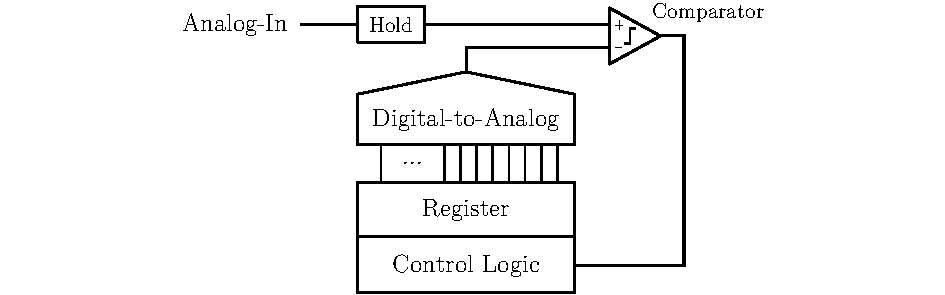
\includegraphics[width=1\textwidth]{diagrams/adc.pdf}
					\caption{Successive-approximation analog-to-digital converter}
					\label{fig:adc}
				\end{figure}
				
				The ADC sampling process takes at least $5\mu{}s$ or approximately 500
				CPU cycles \cite{LPC1768} therefore the CPU should carry out some other
				task while the ADC process takes place. Though an interrupt is provided
				when the ADC completes (and even a direct memory access (DMA) facility
				is provided), this was not used. The temperature sensors will be sampled
				at an extremely low rate (around 2Hz) and latency is not important as
				changes occur very slowly. Instead, a slow-poll is used where the task
				reading from the ADC is suspended for a time typically adequate for ADC
				operation. This system is extremely simple to implement and provides
				adequate read performance.
			
			\subsubsection{Control}
				
				A na\"{i}ve controller could simply turn on the heaters when the
				temperature was below some target temperature or `set point' and then
				off when it met or exceeded it. This controller would cause the
				temperature to overshoot and fall below the set point. Instead a
				proportional-integral-derivative (PID) controller is used which can
				control heaters taking into account such behaviours. These controllers
				are widely used and are often used when a process must be controlled
				which is not completely understood \cite{controleng}.
				
				\begin{figure}
					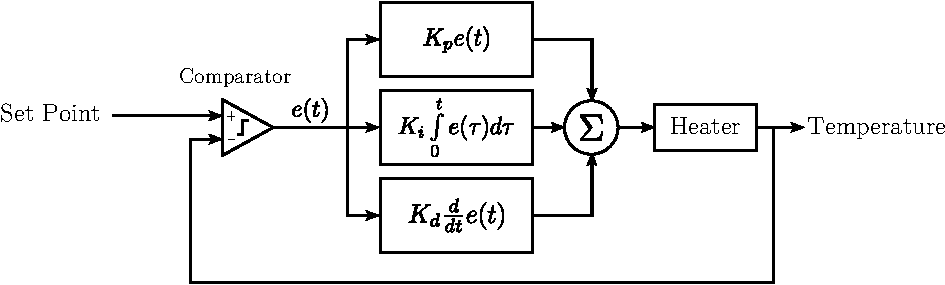
\includegraphics[width=1\textwidth]{diagrams/pid.pdf}
					\caption{PID heater controller schematic}
					\label{fig:pid}
				\end{figure}
				
				Figure \ref{fig:pid} shows a schematic of the PID controller used in the
				system. At time $t$ the comparator calculates the error $e(t)$ between
				the actual temperature and the set point. A value is calculated from
				this error using a factor proportional to the error, the error
				accumulated over time (integral) and the error's rate of change. These
				factors are weighted by the constants $K_p$, $K_i$ and $K_d$
				respectively and then used to control the heater. The three weights must
				be chosen manually to produce sensible behaviour.
				\S\ref{sec:pidtraning} discusses the process of selecting these values.
				
				The value calculated could be used with an analog output or
				PWM\footnote{Pulse width modulation (PWM) is a method of approximating
				analog outputs by rapidly switching a signal on and off with a varying
				duty-cycle. This is cheap to implement in hardware and also avoids
				problems with inefficiencies in MOSFETs when only partially driven.} to
				control the heater or a threshold value used to decide whether a heater
				is on or off (`bang-bang' control). Bang-bang control has been used
				because the previous electronics proved this to be adequate. Using PWM
				to control the heaters may also have resulted in unwanted
				electromagnetic noise.
				
				The PID control loop is executed in its own task at a rate of 2Hz where
				each temperature is read and the heater switched on or off as
				appropriate. Because of the slow rate of change this is an adequate
				response speed. Executing the loop more frequently would not be useful
				and, due to floating point calculations being carried out in software,
				would be costly.
		
		\subsection{Stepper Control}
			
			To drive the TTL stepper controller interface accurately timed pulses must
			be produced to cause the motors to step. These pulses need to be coherent
			so that the three axes can move simultaneously to plot straight paths.
			
			\subsubsection{Timing Constraints}
				
				The stepper controller boards use an Allegro A3982 stepper controller
				which defines the signals and timing requirements. Figure
				\ref{fig:stepperWave} shows an example waveform with 3 forward steps
				followed by 4 backward steps. On the positive edge of each step signal
				the direction is sampled and the stepper controller steps the motor.
				Table \ref{tab:stepperTiming} gives the timing constraints for these
				signals.
				
				\begin{figure}
					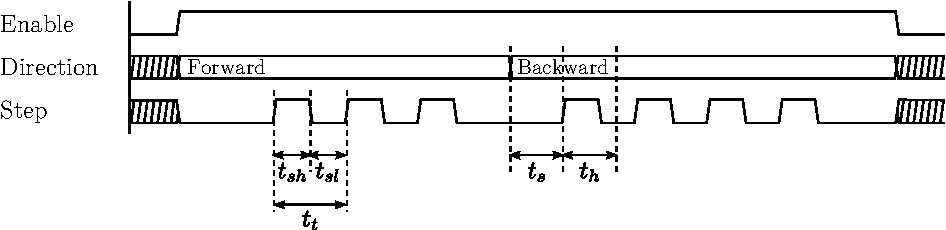
\includegraphics[width=1\textwidth]{diagrams/stepperWave.pdf}
					\caption{Stepper control signal wave diagram}
					\label{fig:stepperWave}
				\end{figure}
				
				% XXX: Step time may be wrong here or in code (here is based on 3300
				% mm/min working fine)
				
				\begin{table}
					\centering
					\begin{tabular}{l l l}
						\toprule
						Period & Meaning & Timing Constraint\\
						\midrule
						$t_{sh}$ & Step high  & $\ge 1\mu{}s$ \cite{allegro} \\
						$t_{sl}$ & Step low   & $\ge 1\mu{}s$ \cite{allegro} \\
						\addlinespace
						$t_{s}$  & Setup time & $\ge 200ns$   \cite{allegro} \\
						$t_{h}$  & Hold time  & $\ge 200ns$   \cite{allegro} \\
						\addlinespace
						$t_{t}$  & Step time  & $\ge 757\mu{}s$ (Experimentally determined) \\
						\bottomrule
					\end{tabular}
					
					\caption{Stepper timing constraints}
					\label{tab:stepperTiming}
				\end{table}
				
				The motors in the printer also add a timing constraint ($t_t$) as they
				are limited as to how often they can step by the mechanical properties
				of the printer. The faster the stepper is driven, the less torque is
				available and the stepper may miss steps or fail to move.
			
			\subsubsection{Timers}
				
				To simplify implementation, Bresenham's line algorithm \cite{bresenham}
				was not used to control the motors. Instead, before the movement begins
				a periodic timer is set based on the frequency at which steps must occur
				and is used to toggle the step signal. Since expensive floating point
				calculations are carried out before each movement in order to convert
				distances in millimetres into numbers steps, the additional calculation
				at the start of a movement is not significant. This scheme therefore
				uses one expensive calculation at the start of the movement followed by
				a small number of inexpensive integer operations on each timer tick.
				
				If a stepper is set to run at its maximum speed, steps will be
				$757\mu{}s$ apart meaning that the signal must be toggled every
				$379\mu{}s$.  Therefore signals may change at up to $1.32\kHz$.
				According to the Nyquist-Shannon sampling theorem a frequency of $f\Hz$
				can only be generated by a timer running at $> 2f\Hz$. This means the
				timer resolution must be above $2 \times 1.32\kHz = 2.64\kHz$ to
				generate such a step signal\cite{shannon}. Intuitively, a timer must
				tick at least twice in a cycle of the desired frequency in order to set
				it high then set it low. Figure \ref{fig:nyquist} shows the result of
				trying to reproduce a signal at $\frac{2}{3}$ ($> \frac{1}{2}$) the
				frequency of the timer resolution and whole cycles can be seen missing
				in the output.
				
				\begin{figure}
					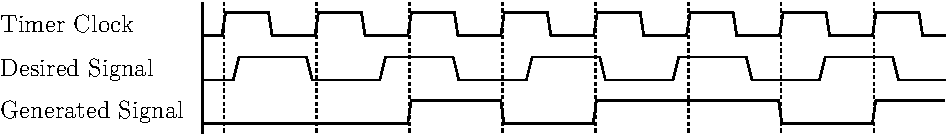
\includegraphics[width=1\textwidth]{diagrams/nyquist.pdf}
					\caption{Nyquist-Shannon sampling theorem example with high-frequency
					signal}
					\label{fig:nyquist}
				\end{figure}
				
				The effect of sampling artefacts can cause further inaccuracies. Figure
				\ref{fig:artefacts} shows a signal below $\frac{1}{2}$ of the sampling
				frequency displaying such artefacts. In the worst case when sampling at
				$f\Hz$, a signal change may be $\frac{1}{f}\s$ late. Therefore,
				increasing the sampling frequency decreases the error introduced by such
				artefacts.
				
				\begin{figure}
					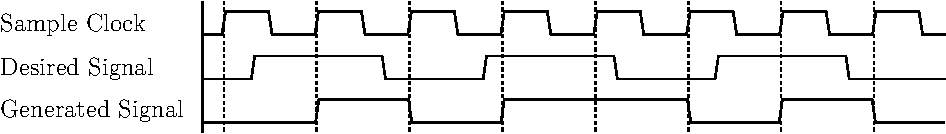
\includegraphics[width=1\textwidth]{diagrams/artefacts.pdf}
					\caption{Example of sampling artefacts}
					\label{fig:artefacts}
				\end{figure}
				
				High print quality depends on smooth, even steps, as a result, the timer
				resolution must be not only above $2.64\kHz$ due to the Nyquist-Shannon
				sampling theorem but also be high enough to reduce sampling artefacts to
				an acceptable level. If errors due to artefacts are to be reduced in the
				worst case to, for example, one-hundredth of the step period then a
				frequency of $264\kHz$ is needed.
				
				FreeRTOS provides timing guarantees for scheduling arbitrary delays
				within tasks. Unfortunately, this uses the system timer which
				ticks at $1\kHz$ which is too far low for the frequencies such as those
				discussed above. Increasing the speed of the system timer would make the
				overhead due to the scheduler running on each tick unacceptable and so
				another timer must be used.
				
				Because the Mbed only provides a limited number of hardware timers, just
				one is used to control all three steppers. As each stepper may not be in
				phase, the time between signals being produced can become very small
				even when the step period is large. This is another example of a
				sampling artefact errors and the resulting errors are again no larger
				than $\frac{1}{f}\s$ for a timer running at $f\Hz$ so no extra timer
				precision is required.
				
				The timers provided on board the Mbed consist of a register comparator
				and counter which is incremented by the system clock after being passed
				through a pre-scaler clock divider (figure \ref{fig:timerArch}). The
				timer was configured such that when the counter matches the register the
				timer is reset and the CPU is interrupted. The pre-scaler is configured
				to increment the counter at $1\MHz$ which exceeds the $264\kHz$
				requirement above.
				
				\begin{figure}
					
\includegraphics[width=1\textwidth]{diagrams/timerArch.pdf}
					\caption{Mbed timer architecture}
					\label{fig:timerArch}
				\end{figure}
				
				The interrupt service routine (ISR) for the timer scans through each
				stepper to determine if its step signal should be toggled and then sets
				the timer compare register to the time the next interrupt should occur.
				
				GCC generates approximately 100 instructions for the ISR taking an
				estimated 250 cycles to execute\footnote{Estimate based on informal
				analysis of the generated assembly code}. Assuming the CPU executes one
				instruction per cycle at $100\MHz$ the amount of CPU time used by the
				ISR in the worst case can be calculated as follows:
				\begin{equation}
					\textrm{Overhead} =
					\frac{\textrm{Interrupts Per Seccond} \times \textrm{ISR Cycles}}
					     {\textrm{CyclesPer Seccond}} =
					\frac{(1.32\times10^3) \times 250}
					     {100\times10^6} = 0.33\%
				\end{equation}
				
				The timer does not drift as it is reset by hardware and continues
				counting while the ISR is executing. The ISR merges steps due within a
				very small period into its current invocation so that when the timer
				compare register is updated the timer will not have reached the old
				value and reset a second time.
			
			\subsubsection{Usage}
				
				An API is provided which allows a number of steps in a given direction
				with a specified period to be sent to a stepper motor. A method which
				blocks until all steps have been completed is also provided. This method
				requests a semaphore which is released by the ISR when all steps have
				been completed. FreeRTOS allows tasks unblocked by the ISR to
				temporarily receive a higher priority during which the task can start
				the next sequence of steps immediately.
		
		\subsection{G-Code Interpreter}
			
			In this subsection, the abstract `G-code machine' is described followed by
			a discussion of which language features are supported and their selection.
			Finally the parser and interpreter will be described.
			
			\subsubsection{The G-Code Machine}
				
				The G-code machine consists of 26 numeric registers named `A' to `Z'.
				A G-code instruction consists of a set of register assignments after
				which the machine evaluates a specific action based on the contents of
				its registers.
				
				Some registers may be reset to an `undefined' state before each
				instruction. This allows the machine to identify when a register is
				written. For example, the `G' and `M' registers are used to specify what
				type of action should occur and if they are not cleared it would not be
				possible to determine which register contains the action required.
				
				Each register accepts either floating point or integer values, for
				example the `G' and `M' registers only accept integer instruction
				numbers while `X', `Y' and `Z' are floating point and accept
				coordinates.
				
				For example, when the instruction \verb|G1 X10 Y-15 Z0.3| is
				encountered, the following register values are set:
				
				\begin{gcoderegs}
					\reg{G}{1}
					\reg{X}{10}
					\reg{Y}{-15}
					\reg{Z}{0.3}
				\end{gcoderegs}
				
				In this example, the action is determined based on the `G' register to
				be `move to' and the `X', `Y' and `Z' registers determine where to move.
				If this is followed by \verb|M104 S225| then the following registers
				will be set:
				
				\begin{gcoderegs}
					\reg{M}{104}
					\reg{S}{225}
					\reg{X}{10}
					\reg{Y}{-15}
					\reg{Z}{0.3}
				\end{gcoderegs}
				
				Note that the `G' register has been undefined but the others have
				remained. In this example, the action is determined based on the `M'
				register to be `set extruder temperature' and the `S' register
				determines the temperature. `X', `Y' and `Z' are ignored. Finally, if
				\verb|G1 Z0.6| is encountered the following registers are set:
				
				\begin{gcoderegs}
					\reg{G}{1}
					\reg{S}{225}
					\reg{X}{10}
					\reg{Y}{-15}
					\reg{Z}{0.6}
				\end{gcoderegs}
				
				Once again the machine determines the action to be `move to' and moves
				to the position defined by `X', `Y' and `Z' ignoring the `S' register.
				Because the values of `X' and `Y' have not been changed the machine will
				only move the `Z' axis.
			
			\subsubsection{Feature Subset Selection}
				
				G-code interpreters support a large variety of features ranging from
				comments and instructions which return data to error checking and simple
				flow control. As well as various language features, the actions
				available and the way they use the values in each register differ.
				
				To keep the system as simple (and fast) as possible only features and
				actions required by the Skeinforge G-code generator were implemented.
				The resulting language simply supports comments and writing to registers
				but none of the more advanced features supported by some interpreters.
				The syntax supported is given in Backus-Naur Form (BNF) in appendix
				\ref{sec:gcodebnf}.
				
				Actions (and their treatment of registers) were also selected based on the
				output of Skeinforge and include:
				\begin{itemize}
					\item Unit selection
					\item Calibration
					\item Movement
					\item Motor control
					\item Power control
					\item Temperature control
					\item Waiting for heaters to warm-up
					\item Timed pauses
				\end{itemize}
				A complete list of actions supported are enumerated in appendix
				\ref{sec:gcodeactions}.
			
			\subsubsection{Parsing}
				
				The G-code subset supported is very simple and it is simpler to
				implement the parser by hand than to use a standard parser generator
				such as GNU Bison. Such tools also generate code that is not optimised
				for running on a microcontroller in a real-time environment.
				
				A simple state machine was built by hand which parses and executes the
				G-code setting and reading registers as described above. If unexpected
				characters or register values are encountered a flag is set and the
				parser continues from the next character or instruction. The state
				machine is given in appendix \ref{sec:stateMachine}.
		
		\subsection{System Control}
		
		\subsection{Network Interface}
			
			\subsubsection{G-Code}
			
				\subsubsection{TCP}
				
				\subsubsection{UDP}
			
			\subsubsection{Status}
	
	\section{Utilities}
		
		\subsection{G-Code Sender}
		
		\subsection{Status Monitoring}
	
	\section{Safety}
		
		\subsection{STOP Button}
		
		\subsection{Watchdog}
		
		\subsection{Power-on Behaviour}
	
	\section{Methodology}
		
		\subsection{Tools}
			
			\subsubsection{Git (Version Control)}
			
			\subsubsection{Wireshark (Network Protocol Analyser)}
		
		\subsection{Languages}
			
			\subsubsection{C}
			
			\subsubsection{Python}
		
		\subsection{Debugging}

	\chapter{Testing \& Evaluation}
	
	% TODO: Z-Axis slipping (add to hitting self)
	
	\label{sec:testing}
	
	In this chapter the tests carried out during development are described along
	with an evaluation of the results. Each section describes the major components
	of the system concluding with an evaluation of the system's overall
	performance.
	
	\section{Electronics}
		
		The major components of the electronics were prototyped and tested on a
		breadboard using a multimeter. The higher power components, such as the
		heaters and motors, were initially disconnected until the circuit was deemed
		to be working. Once connected, these components were then tested with
		careful supervision to ensure that they functioned correctly and that the
		current flowing through each part of the circuit was as expected. The tested
		circuit designs were then built on circuit boards where the connections were
		tested for continuity and checked for short circuits.
		
		Overall the electronics performed well and no problems caused by electrical
		noise were observed. A few parts of the system were found to exhibit
		unexpected behaviour and these are outlined in the following subsections.
		
		\subsection{MOSFETs}
			
			After an extended period of being powered on the MOSFETs became hot
			running at around 50\dC. The data sheet for the IRLU8729PbF MOSFETs states
			that the operating temperature range is from $-55\dC{}$ to 175\dC and so
			this temperature is safely within operational limits.
			
			% TODO: Why does this happen?
		
		\subsection{End-stops}
			
			Printed plastic paddles were originally planned as the triggers for the
			end-stops. Unfortunately, acrylonitrile butadiene styrene (ABS) plastic
			used by the Makerbot is transparent to the infra-red wavelengths used by
			the opto-interrupters and so this material is unsuitable. The design was
			changed to instead use wooden craft `lollipop sticks' which fit into
			pre-cut slots in the Makerbot and easily trigger the opto-interrupters.
		
		\subsection{ATX PSU}
			
			Some ATX PSUs require a certain load on all provided voltages in order to
			power up properly \cite{reprapatx}. While a large load is drawn on the 12V
			line for the heaters and motors, the 5V line only powers the Mbed which
			draws little power. The result of this is that the 12V line attached to
			the heaters only provided 9V and so could not warm up to the required
			temperature.
			
			A resistor can be added to the 5V line to draw extra current and fully
			power up the PSU \cite{reprapatx}. Due to time constraints an alternative
			PSU was used which did not feature this fault rather than modifying the
			circuit.
	
	\section{FreeRTOS}
		
		The availability of the FreeRTOS port made it extremely easy to integrate
		into the project. FreeRTOS itself provided the right balance of features and
		performance for the project. The operating system did not place restrictions
		on the use of low-level system registers and simply provided preemptive
		multitasking and some atomic operations as required.
		
		The operating system was initially tested for timing accuracy using a
		frequency probe attached to an I/O pin toggled by a simple demonstration
		program to ensure the system was behaving as expected. This test yielded a
		mismatch from the expected frequency which was found to be an incorrect
		definition of the clock speed. Once fixed the system ran as expected running
		the included demo programs as defined. No further issues were found during
		the course of the project.
	
	\section{\uIP{} \& Networking}
		
		% XXX: Restructure this section
		
		Various tests were conducted on the \uIP{} stack during the project,
		initially concentrating on performance and, upon discovery of the flow
		control problems, moving on to testing the system's correctness. This
		section discusses these tests and concludes with an evaluation of its
		suitability for the project.
		
		% TODO: Talk about performance tests
		
		\label{sec:udpPerformance}
		
		Wireshark was used to monitor the packets sent between the Mbed and computer
		and it became apparent that every packet was being received from the Mbed
		twice. After ruling out network problems being the cause, the bug was traced
		down to the Ethernet driver provided by the demo. The driver duplicated
		every IP packet sent to the network (including IMCP Ping Requests, figure
		\ref{fig:ping}). As well as wasting bandwidth, when a TCP packet
		acknowledgement (ACK) from the Mbed gets delayed in the network
		retransmission will result in there being four duplicate ACKs in the
		network. This causes the sending computer to retransmit and incorrectly
		adjust its expectations of the network connection \cite{duplicateack}. This
		behaviour is one factor that can prevent TCP flow control from functioning
		correctly.
		
		%TODO: Get actual shot!
		\begin{figure}
			\begin{verbatim}
				$ ping 192.168.3.100
				PING 192.168.3.100 (192.168.3.100) 56(84) bytes of data.
				^C
				--- 192.168.3.100 ping statistics ---
				2 packets transmitted, 0 received, 100% packet loss, time 1006ms
			\end{verbatim}
			\caption{Ping responses being duplicated by \uIP{} driver}
			\label{fig:ping}
		\end{figure}
		
		The packet duplication behaviour is often added to to work around problems
		caused by \uIP{} only allowing one packet to be sent before waiting for an
		acknowledgement \cite{allpacketsdup}. Modern systems (such as Windows and
		Linux) will allow several packets to arrive before acknowledging them all at
		once, saving bandwidth. If only one packet is sent then the ACK won't be
		sent back immediately, delaying the transmission of the next packet by
		\uIP{}. By duplicating each packet, the receiver is forced to immediately
		send an ACK as, from receiver's perspective, a duplicate packet may indicate
		that the original packet was delayed in the network and the sender did not
		receive an ACK in time (because the receiver had not received it). As a
		result the receiver has to send the ACK immediately allowing the next packet
		to be transmitted by \uIP{}.
		
		Though this wastes bandwidth it reduces the wait between each packet being
		sent and dramatically increases the bandwidth available from the Mbed to the
		computer. Disabling this work-around means sending multiple-packet bursts of
		data from the Mbed is more time consuming but removes a barrier to flow
		control being used successfully. The only data sent from the Mbed are status
		responses which are small enough (around 30 bytes) to fit in a single
		packet. Disabling packet duplication, in favour of removing a barrier to
		proper flow control, is a good trade off.
		
		\label{sec:tcpProblem}
		
		Unfortunately, problems with flow control persisted with no improvement
		after disabling packet duplication. With the duplicate packets removed, the
		problem became clearer. TCP sends a window size with each packet
		representing the amount of data the receiver is still able to receive.
		\uIP{} reports a constant window size until the method \verb|uip_stop()| is
		called when the window size is set to zero and any further packets received
		are discarded (and the zero window message resent) until
		\verb|uip_restart()| is called and the old window size is restored and a
		packet sent to the computer to request data transfer to continue. This
		allows the system to stop receiving data when the G-code buffer is too full.
		
		To test this a program was generated which contained a long sequence of
		small movement commands. This would allow the buffer to initially fill up
		and then be constantly kept topped up by the computer. The actual behaviour
		is shown in figure \ref{fig:uIPFlowControl}. The buffer is initially filled
		(the first spike) but then the sender waits an exponentially growing period
		until it starts filling the buffer again regardless of when the window size
		is made non-zero.
		
		\begin{figure}
			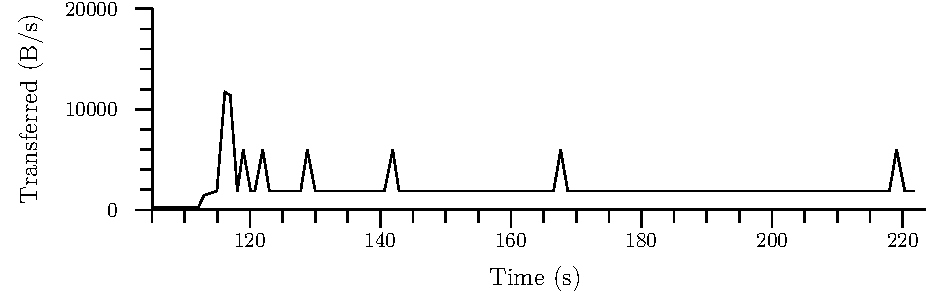
\includegraphics[width=1\textwidth]{diagrams/uIPFlowControl.pdf}
			\caption{Exponential back-off by computer when \uIP{} flow-control used}
			\label{fig:uIPFlowControl}
		\end{figure}
		
		By inspecting the packets sent and received, the window size is always
		obeyed but the packet announcing the window size becoming non-zero appears
		to be ignored. Wireshark's protocol checker did not report any errors and
		comparison with the known-working implementation in Linux did not reveal any
		fundamental differences. Unfortunately further study did not yield a
		diagnosis for the problem. Due to the time constraints imposed by the
		project TCP had to be dropped for G-code transmission in the project.
	
	
	\section{Temperature Readings}
		
		The temperature readings depended on correct values being read from the
		analog inputs and on correct calculation of the temperature based on these
		readings. Though consistency is important, reading temperatures close to the
		actual value is relatively unimportant as the temperature is fairly uneven
		within the heated components of the printer. The temperature values used
		during printing will be calibrated manually and the actual temperature in
		\dC{} is not significant but the consistency with which it is reached is.
		
		To test analog input, a selection of resistors with known values within the
		range of values the thermistor could exhibit were tested. As well as
		breadboard testing, the test was repeated on the final circuit board as the
		screw terminal used to connect the thermistors could also be used to connect
		a test resistor directly.
		
		When converted to a resistance using (\ref{equ:potdiv}), the values read
		were found to be within $\pm2\%$ of the resistor value as read by a
		multimeter (a difference which is accounted for by the fact that a second
		resistor with a $\pm5\%$ tolerance is used in the potential divider).
		
		To test that temperatures were being correctly converted from the resistance
		of the thermistors, an infra-red thermometer (figure \ref{fig:thermometer})
		was used to take temperature readings from the extruder and platform and
		these values were then compared against the value calculated using
		(\ref{equ:steinhart}). The heaters were turned on and readings were taken
		every minute as the extruder and platform heated up and then every five
		minutes for half an hour as it cooled down. The tests were repeated multiple
		times alongside other experiments, each time with similar results, to ensure
		consistency.
		
		The radius of the area measured by the thermometer becomes larger as it is
		moved further away from the target. Because the temperature across the
		platform and extruder vary greatly depending on location, the thermometer
		was placed close to the centre of the extruder nozzle and the centre of the
		build platform.
		
		\begin{figure}
			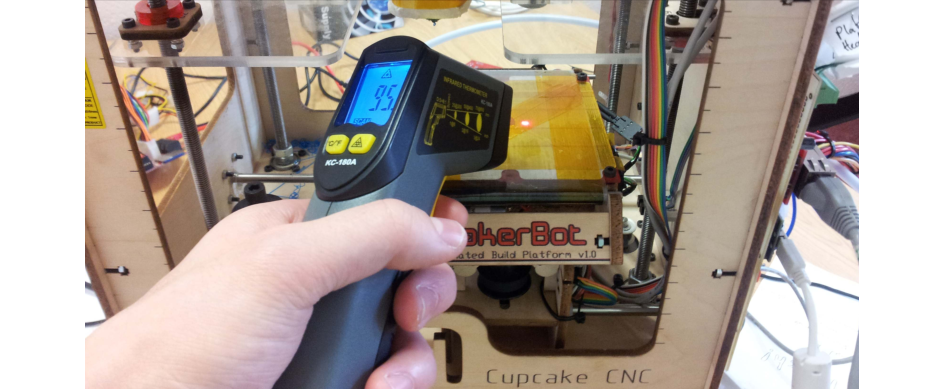
\includegraphics[width=1\textwidth]{diagrams/thermometer.pdf}
			\caption{Checking platform temperatures using an infra-red thermometer}
			\label{fig:thermometer}
		\end{figure}
		
		The temperatures recorded for the extruder were within $\pm1\dC$ below
		100\dC{} but rose to around $+8\pm1\dC$ around 220\dC{} (normal operating
		temperature).
		
		The platform temperatures were initially incorrect by $\pm10\dC$ or more.
		The platform contains a built in potential divider which was not used by the
		design (instead using the circuit on the main board) and was found to be
		connected to the main board. Once the connections were corrected, readings
		followed a similar pattern to the extruder (up to the 125\dC{} the platform
		is designed to operate at).
		
		The results above represent adequate performance for the task of maintaining
		a desired temperature and also show that the temperatures read are close to
		their real values such that an operator can safely tell from a temperature
		reading that the device is unsafe to touch.
	
	\section{PID Control}
		
		% XXX: Yeah...
		
		\label{sec:pidtraning}
		
		The PID controller has three constants ($K_p$, $K_i$ and $K_d$) which must
		be manually tuned to yield sensible system performance. While operating, the
		temperature oscillates around the set point. An optimal system has
		oscillations that are as small as possible and which responds as quickly as
		possible to changes in the set point or environment.
		
		PID controller tuning is a non-trivial problem for which automated solutions
		are either highly specialised or unavailable. Heuristics exist such as The
		Ziegler-Nichols method for selecting good values which work in many cases
		and require human interpretation \cite{ziegler}.
		
		% XXX: Jump?
		
		The Makerbot wiki suggests values (given in table \ref{tab:makerbotpid}) as
		a starting point requiring only a small amount of adjustment
		\cite{makerbotpid}. After selecting these values the printer's performance
		was monitored both while idle and during printing and the size of
		oscillations were measured. Performance was similar while in both states
		(with a temperature jump in platform temperature at the start of printing
		when molten plastic is extruded directly on to the platform). Oscillations
		were $\pm2\dC$ for the extruder and platform. Though this is greater than
		the $\pm1\dC$ recommended, print quality was not adversely effected.
		
		\begin{table}
			\centering
			\begin{tabular}{l l l}
				\toprule
				Constant & Extruder Value & Platform Value \\
				\midrule
				$K_p$    & $5.143$        & $7.0  $  \\
				$K_i$    & $0.0612$       & $0.342$ \\
				$K_d$    & $108.0$        & $36.0 $  \\
				\bottomrule
			\end{tabular}
			
			\caption{Generic PID controller constants for a Makerbot
			         \cite{makerbotpid}}
			\label{tab:makerbotpid}
		\end{table}
	
	\section{Stepper Control}
		
		The stepper control system consists of code for producing accurately timed
		steps and code for coherently moving the stepper motors. These two parts
		were tested separately as described in the following subsections. Finally,
		the results of these tests are evaluated.
		
		\subsection{Timing}
			
			To ensure timing accuracy, the three stepper signals were driven at a
			combination of frequencies with a frequency meter attached to the step
			pin. These tests were generated initially using a program on the
			microcontroller (so that the system was not under any load) and then using
			G-code sent over the network interface while other requests were being
			made (to place the system under reasonable load).
			
			The frequencies measured were exact to within the accuracy of the meter
			(four significant figures) for all tests.
			
			% XXX: What does that really mean?
			
		
		\subsection{Stepping}
			
			To test that stepping was happening coherently, with sequences of steps
			correctly spaced apart, the system was connected to the printer and
			circles were plotted on the axes. The circles are made up of short,
			continuous line segments where the relationship between the movements on
			each axis is not constant. Once again, the test was initially carried out
			using a test program running on the Mbed and then by G-code sent over the
			network. The number of segments the circle was divided into was increased
			from $30$ to $3,000$ and the speed set to $330\mm/\s$ and $3300\mm/\s$ to
			test slow and fast movements.
			
			The performance of the system was measured by visual inspection of the
			movement and circles plotted by attaching a pen to the extruder. The time
			taken the plot the circles was also measured using a timer on the Mbed to
			see if the overhead between each segment caused significant drift. Above
			around $100$ segments the circles drawn appeared smooth and at low and
			high speeds the overhead after 20 circles had been plotted at each speed
			and resolution was less than the $1\ms$ resolution of the timer. Finally,
			to ensure that steps were not being missed the system was homed to a known
			point between tests and this did not drift after all tests had completed.
			
		\subsection{Evaluation}
		
			The amount of plastic deposited at a given point during a print is
			dependent on the rate at which the plastic is extruded and also the rate
			at which the platform moves. The accuracy of the timing (combined with the
			mechanical properties of the machine) determines the platform's rate of
			movement. The print quality therefore depends on these factors.
			
			% XXX: Quantify
			
			The timing accuracy measured above indicates that errors caused by timing
			will be far smaller than the mechanical errors in the system. The
			inspection of the system actually stepping indicates that there is no
			significant timing drift caused by processing between movements. The tests
			also showed that the system can easily deal with plotting sub-millimetre
			paths.
	
	\section{End-stops}
		
		The endstops were tested under various lighting conditions to observe the
		effect on the opto-interrupters. The following lightings conditions were
		tested:
		\begin{itemize}
			\item Ambient strip lighting
			\item Ambient halogen lighting
			\item Ambient incandescent lighting
			\item Ambient natural light
			\item Direct halogen lighting
			\item Direct incandescent lighting
			\item Darkened room
		\end{itemize}
		
		Testing consisted of interrupting each opto-interrupter by moving the
		printer axes so that the end-stop should be triggered and observing the
		digital value read by the Mbed and the state of the debugging LED. Under all
		but the direct lighting conditions the correct value was read and the
		debugging LEDs were completely off or completely on. Under direct lighting,
		especially incandescent lighting, the state read by the Mbed for some
		end-stops was stuck where external light shone into the opto-interrupter. In
		these cases the debugging LEDs did not become completely `off' indicating
		that the opto-interrupter was being triggered.
		
		Though these results suggest that the end-stops cannot be used under direct
		lighting from halogen or incandescent bulbs, the system was found to perform
		well outside these conditions. Although not tested (due to unfavourable
		weather conditions), direct natural light may also have caused similar
		problems.
		
		% TODO: Moved to conclusions
		
		%To solve this problem, a more complex system can be implemented. The
		%infra-red LEDs in the opto-interrupters are pulsed by the microcontroller
		%and the photo-transistor's current is checked for the presence of these
		%pulses. External light sources are unlikely to contain the same pulses and
		%so the system can be sure of the origin of the light passing onto the
		%photo-transistor. Unfortunately this would require significant additions to
		%the electronics and a change to the end-stop interface. As a result, the
		%changes could not be made within the time frame of project. Instead the
		%printer should be used out of direct light to ensure that the end-stops
		%operate correctly.
	
	\section{Buffer Utilisation}
		
		To ensure that the printer did not stall during regular print jobs, the
		G-code and low-level command buffers were monitored during the execution of
		various test jobs. Buffer underruns or low buffer utilisation could indicate
		a performance issue in the G-code interpreter, network interface or their
		interaction with the operating system.
		
		The utilisation and size of each buffer along with a counter for the number
		of underruns experienced by the command-buffer are logged while various
		G-code files are sent to the printer. The test files consisted of:
		
		\begin{description}
			
			\item[Circle drawing with low detail] This test ensures that given a
			sequence of slow G-code instructions the printer keeps all buffers
			reasonably full and that the network interface can cope with infrequent
			small bursts of data.
			
			\item[Circle drawing with high detail] This test ensures that given a
			constant sequence of fast G-code instructions the printer keeps all
			buffers reasonably full and that no underruns occur during busy periods.
			
			\item[Circle drawing with high detail and pauses] This test ensures that
			given a sequence of fast G-code instructions separated by sleeps where the
			buffers filled and the network interface paused can quickly restart after
			the sleep.
			
			\item[Test box model] This non-synthetic test is a simple print job which
			contains long pauses (during heating and cleaning phases), relatively
			low-activity periods (border drawing) and reasonably detailed periods
			(fill patterns).
			
		\end{description}
		
		% TODO: Results
	
	\section{System Testing}
		
		The system was tested as a whole to assess its performance in both synthetic
		printing benchmarks and tests as well as printing real-world objects. These
		tests also aid in calibration of the G-code generator (Skeinforge). The
		synthetic tests allow the printer's performance to be objectively measured
		while real objects show real-world performance of the printer in its
		intended application.
		
		\subsection{Synthetic Tests}
			
			As a simple test of using all of the printer's components coherently, the
			circle plotting test was modified to produce spirals and the heaters and
			extruder enabled. Figure \label{fig:syntheticTests} shows samples of the
			output of these tests:
			\begin{description}
				
				\item[(A)] The extruder was moved at a safe distance from the platform
				to ensure that all components move together but without the risk of the
				extruder colliding with the platform or blocking the nozzle of the
				extruder.
				
				\item[(B)] As in (A) but the extruder is moved closer to the platform to
				test that the system can safely operate next to the platform and that
				the plastic adheres to the platform (and then properly detaches when
				ejected).
				
				\item[(C)] A larger spiral printed to test that the plastic adheres
				closer to the (colder) edges of the platform and that warping due to
				temperature changes during the print does not cause problems.
				
				\item[(D)] The winding of the spiral is tightened to test that the
				plastic adheres to itself and the platform and that warping does not
				cause the print to fail. Figure \ref{fig:looseSpiral} shows a print
				where the spiral was printed too loosely and it did not adhere to
				itself.
				
			\end{description}
			
			\begin{figure}
				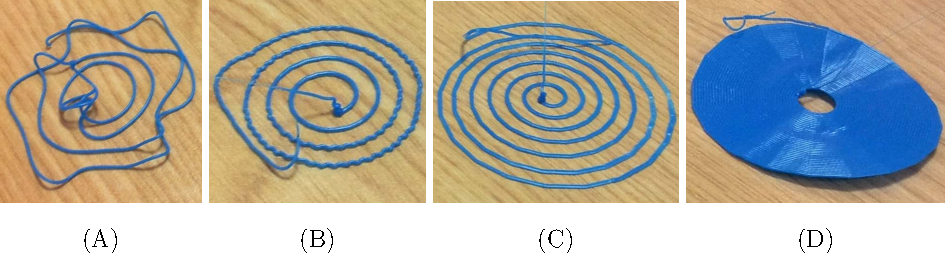
\includegraphics[width=1\textwidth]{diagrams/syntheticTests.pdf}
				\caption{Synthetic 3D printer tests for basic calibration}
				\label{fig:syntheticTests}
			\end{figure}
			
			\begin{figure}
				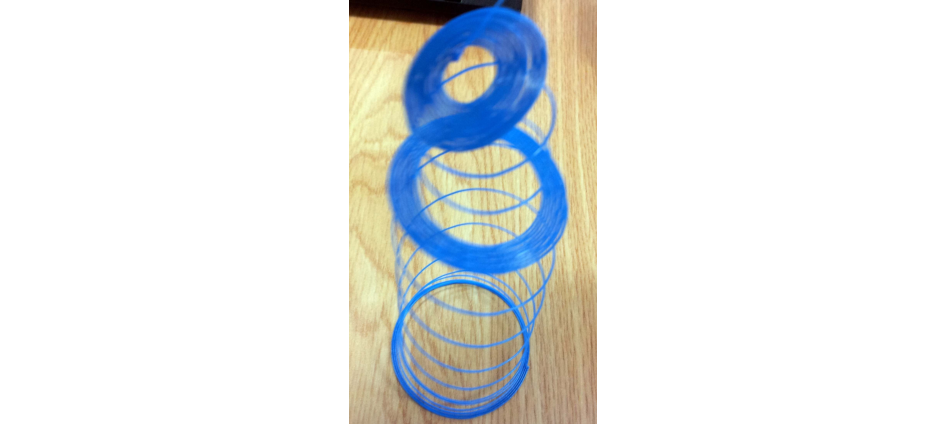
\includegraphics[width=1\textwidth]{diagrams/looseSpiral.pdf}
				\caption{Bad print of the test in figure \ref{fig:syntheticTests}(D)}
				\label{fig:looseSpiral}
			\end{figure}
			
			These prints were repeated, varying the platform temperature, Z-axis
			position (height) and the tightness of the spiral until the tests
			performed as described above. These tests ensure that the printer is
			capable of operating all its major components coherently in order to
			produce printed object.
			
			To test the system with G-code generated by Skeinforge, a simple 3D model
			of a cuboid (Figure \ref{fig:testCubes} (A)) was printed. This print
			yields a cuboid of known dimensions and is used to check calibration
			settings for Skeinforge. The cuboid is initially printed on top of a thick
			`raft' of plastic (used to ensure an even printing surface) and then
			separated using a chisel.
			
			The dimensions of the cuboids were checked using a pair of digital
			calipers (figure \ref{fig:calipers}) to ensure that the printed object is
			of the correct size. The Makerbot wiki claims that $0.1\mm$ resolution is
			possible on a correctly tuned machine and this requirement was met by most
			of the printed cuboids \cite{makerbotfaq}. In a small number of cases, the
			Z-axis of the printer did not move the required amount due to the
			mechanism jamming, a known problem with the Makerbot design
			\cite{zaxisissue}. As a result, these prints were of the incorrect height
			but were otherwise correct and the problems not attributed to the
			firmware.
			
			\begin{figure}
				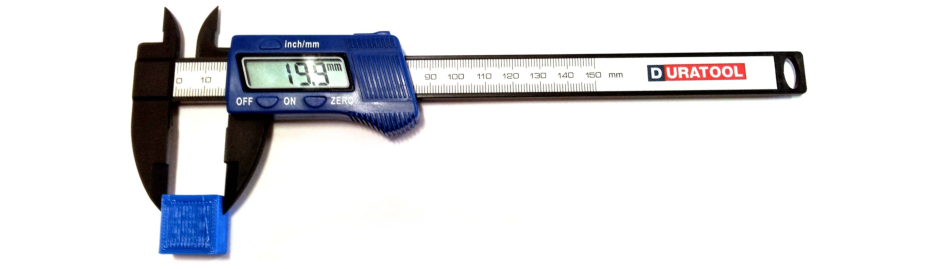
\includegraphics[width=1\textwidth]{diagrams/calipers.pdf}
				\caption{Digital calipers used for measuring test cuboids}
				\label{fig:calipers}
			\end{figure}
			
			\begin{figure}
				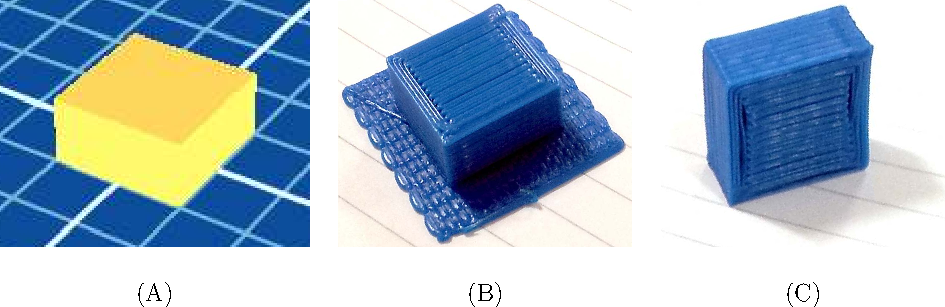
\includegraphics[width=1\textwidth]{diagrams/testCubes.pdf}
				\caption{Test cuboid model (A) print from Skeinforge G-code before raft
				         removal (B) and after raft removal (C)}
				\label{fig:testCubes}
			\end{figure}
			
		
		\subsection{Test Objects}
			
			To test the printer's ability to produce useful objects, various objects
			were printed including objects with moving parts and objects near the
			print-size limits for the printer. These tests check the system's ability
			to deal with large and complex loads. A selection of printed test objects
			is provided in Appendix \ref{sec:examplePrints}.
			
			\subsubsection{Detailed Prints}
				
				Prints with detailed areas were used to test that the system could
				process the larger density of G-code at the required rate and also to
				ensure that steps were not missed during printing.
				
				For example, figure \ref{fig:vase} shows a vase which yields very short
				line segments while printing the corners of the shape. The previous
				electronics would not be able to process this design fast enough and
				would skip instructions causing steps to be missed. With the new
				electronics no buffer underruns or printing problems occurred during a
				run featuring a large version (shown) and a smaller version containing
				finer detail as a result.
				
				\begin{figure}
					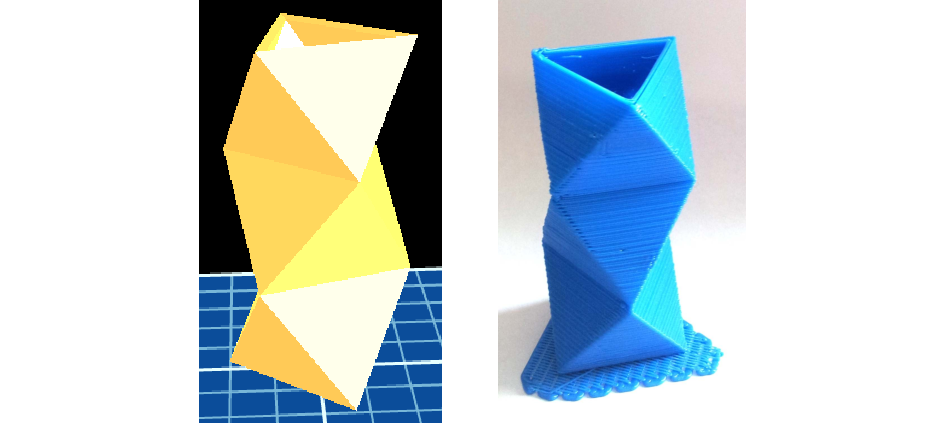
\includegraphics[width=1\textwidth]{diagrams/vase.pdf}
					\caption{3D printed vase with detailed corners}
					\label{fig:vase}
				\end{figure}
			
			\subsubsection{Large Prints}
				
				% XXX: No objective numbers...
				
				Large prints stress the printer and electronics for long periods and can
				reveal missed motor steps or instructions. The previous system had
				frequent issues printing large objects due to skipped instructions or
				steps and is a particular area for improvement.
				
				Of the large objects printed, only one failed to print (figure
				\ref{fig:failedPrint}). This was due to the object warping (A) and
				becoming detached from the platform during the print causing the tip of
				the extruder to rip the object off the platform (B). Unevenness in the
				temperature of the object during printing is the cause of this
				distortion. This is partially caused by unevenness in the temperature of
				the build platform. Unfortunately, this is a problem with the printer's
				design which is not addressed in this project.
				
				\begin{figure}
					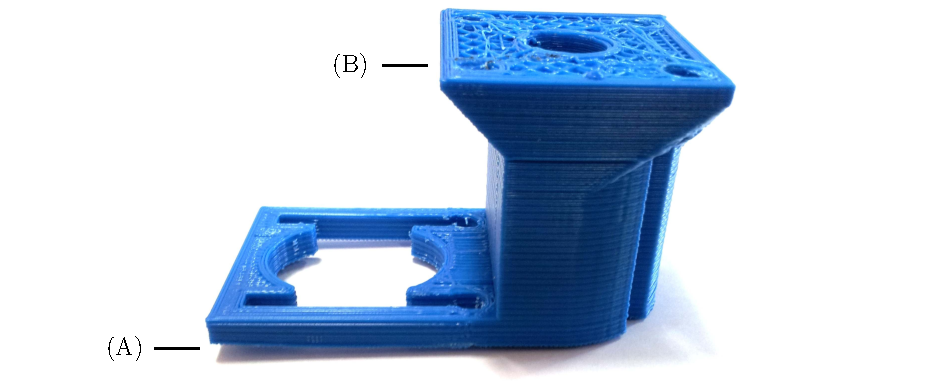
\includegraphics[width=1\textwidth]{diagrams/failedPrint.pdf}
					\caption{Failed large print showing warping (A) and a collision with
					         the extruder (B)}
					\label{fig:failedPrint}
				\end{figure}
				
				% XXX: Conclude...?
			
			\subsubsection{Raftless Printing}
				
				Though the first prints were completed on top of a raft, it was later
				disabled. This reduced print time, improved print quality and allowed
				intricate designs such as a comb to be printed (figure \ref{fig:comb})
				where removal of the raft would damage the design.
				
				\begin{figure}
					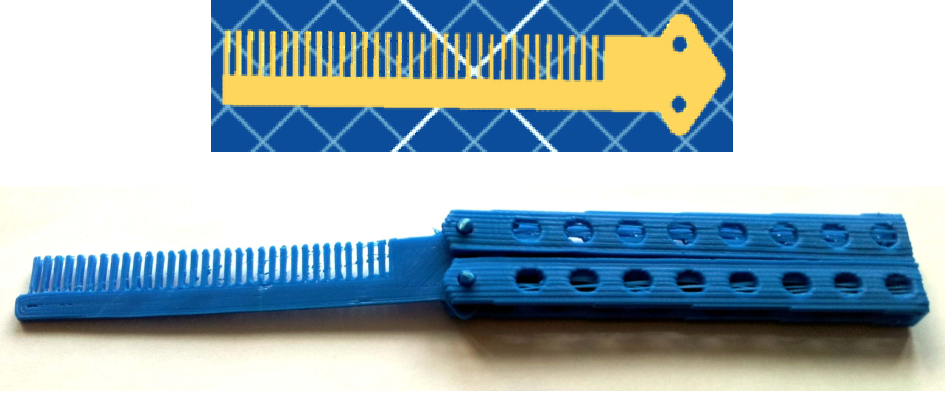
\includegraphics[width=1\textwidth]{diagrams/comb.pdf}
					\caption{Folding `butterfly comb', printed without a raft (designed by
					         techno246 \cite{butterflycomb})}
					\label{fig:comb}
				\end{figure}
				
				Many objects were reprinted using raftless printing and performance was
				generally similar with the exception of larger designs. These
				experienced greater warping without the support of the raft and thus
				were more prone to failure due to the extruder hitting the object.
				
				% XXX: Conclude

	\chapter{Conclusions \& Future Work}
	
	\label{sec:conclusions}
	
	% XXX: Eeek
	In this chapter, the outcomes of the project are compared against the initial
	goals. Finally, future work based on things learnt from the project and the
	limitations of the system is suggested.
	
	\section{Project Goals}
		
		The three project aims have each been addressed within the project and in
		this section the degree to which they have been met is described.
		
		\subsection{Electronics}
			
			The new electronics functionally replace all the features of the old
			electronics and have proved reliable in testing.  With a single board the
			system is also a lot simpler than the previous three boards (featuring a
			custom communications protocol and extra microcontroller).  Though not
			quite as polished as a printed circuit board (PCB), it offers a reasonable
			amount of space for future expansion. The
			
			The solid state MOSFETs, used for heater control, have performed well with
			the silent operation notable over the previous system. They also allow the
			possibility of variable power control with only software changes.
			
			The only notable issue remaining with the electronics is its compatibility
			with certain ATX PSUs. Despite the simplicity of the fix, time was not
			available to implement and test the change. Future work should aim to
			address this issue.
		
		\subsection{Firmware}
			
			% TODO: Mbed debugging difficulties
			
			The firmware written for the Mbed proved to be an improvement over the
			previous system making more detailed prints possible. It is also far more
			modular in design making expansion and experimentation feasible. The print
			quality achieved by the printer is now consistent with the constraints of
			the hardware itself rather than inadequacies of the firmware.
			
			FreeRTOS proved a good choice for the operating system as it provided a
			reliable multi-process environment. It also didn't place any restrictions
			on development allowing straightforward code for interacting with the
			low-level features of the Mbed.
			
			\uIP{}, with the exception of the TCP flow control issue, was well suited
			to the project providing the features needed allowing straightforward
			development. As well as this, the API it enforces (requiring protothreads
			and protosockets) is likely to make future expansion of the network
			interface difficult due to it's heavy restrictions. Future changes to
			overcome these problems are discussed in \S\ref{sec:future_network}.
			
			The stepper and heater control systems were adequate for this project
			though relatively na\"ive. Possible future improvements are described in
			\S\ref{sec:future_firmware}.
		
		\subsection{End-stops}
			
			Though susceptible glitches under direct lighting, the end-stops developed
			functioned correctly and allowed automatic calibration of the axis
			positions as required. They also obey the standard interface used by other
			Makerbot end-stops meaning future modifications may make use of standard
			designs.
			
			The need to build a control circuit resulted in another circuit board on
			the printer reducing some of the simplicity gained from simplifying the
			main electronics. The CAT-5 cables used to connect to the rest of the
			electronics are also bulky, especially considering that only a single
			signal wire is contained within each cable.
			
			Due to time limitations, the end-stops are not used except for
			positioning. There are other uses for the sensors which are described in
			\S\ref{sec:future_endstop}.
		
	\section{Future Work}
		
		There are many possible avenues of future work which would either strongly
		complement the results of this project or build directly on the system. The
		most interesting of these possibilities are presented below.
		
		\subsection{Network Interface}
			
			\label{sec:future_network}
			
			The interface with the printer is an important part of the system.
			Unfortunately, the interface built falls short in some areas and these
			issues are deserving of further work.
			
			\subsubsection{G-code Interface}
				
				No job control, security or multiple-user support is provided by the
				G-code interface of the printer. Each of these problems restricts the
				printer to networks of trusted users who are able to manually
				collaborate when scheduling print jobs. Future work might build upon
				conventional printer interfaces, for example integrating with CUPS, to
				extend the work already done in this area.
			
			\subsubsection{Network Stack}
				
				Due to the limitations and bugs in \uIP{} an alternative stack such as
				lwIP could be used \cite{lwip}. This would provide a higher level,
				FreeRTOS-integrated network interface and enable TCP to be used for
				G-code transmission. This improved interface could also make other
				improvements to the network interface significantly cleaner.
			
			\subsubsection{Web Interface}
				
				The Mbed is powerful enough to generate and host dynamic web pages. A
				web application for control and monitoring of the printer via a web
				interface could make the printer significantly easier to use.
		
		\subsection{Endstop Support}
			
			\label{sec:future_endstop}
			
			To eliminate problems caused by lighting, a more complex system could be
			implemented.  The infra-red LEDs in the opto-interrupters could be rewired
			such that they can be pulsed by the microcontroller. The
			photo-transistor's signal is then checked for the presence of these
			pulses. External light sources are unlikely to contain the same pulses and
			so the system can be sure of the origin of the light passing onto the
			photo-transistor.
			
			As well as this, the end-stops could be used for safety to detect when the
			axis have moved outside their operating area unexpectedly. This could help
			prevent damage to the printer when G-code with unreachable coordinates are
			used.
			
		\subsection{G-Code Support}
			
			The subset of G-code supported by the printer is limited to that produced
			by Skeinforge. To allow other tools to be used for G-code generation and
			also to allow more features of the printer to be exposed, the G-code
			support could be extended.
		
		\subsection{Firmware Improvements}
			
			\label{sec:future_firmware}
			
			% TODO: Cite motion compensation
			
			Complex stepper control systems don't often step at a constant rate.
			Instead the speed is increased and decreased gradually which takes
			advantage of stepper motors' increased talk at low speeds. Such a system
			would also require more precise control of the extruder as the amount of
			plastic required would vary throughout each line segment.
			
			% TODO: Cite PID hardness with variable power
			
			The heaters could potentially respond more appropriately if variable
			amounts of power could be supplied (rather than just `on' and `off'). This
			requires PWM support to be added to allow the heater to be controlled
			variably. PID controllers often require complex additions to enable
			control of such systems and require careful set up.
			
		\subsection{Mechanical Improvements}
			
			As well as the aspects focused on in this project, many improvements can
			be made by modifying the printer's mechanical components. This work is the
			focus of many hobbyists and organisations with improvements in further
			generations of Makerbot being made. Porting promising ideas from other
			printers could provide valuable improvements in performance.
			
			% XXX: Expand?

	
	% End matter
	\bibliography{refs}
	
	% this determines the style in which the references are printed, other
	% possible values are plain and abbrv
	\bibliographystyle{alpha}
	
	% Appendices
	\appendix
	\chapter{Example Printing Workflow}
	
	The following appendix contains a walk-through of the complete process of
	designing and printing an object from scratch. The process begins with the
	production of a 3D model of the design. The next step is to convert the model
	into G-code instructions and send them to the printer. A description is then
	given of the key phases of the printing process. Once the print is complete,
	the printed object is finished after a small amount of cleaning up if
	required.
	
	A simple cuboid is used as an example throughout as the process of designing
	complex 3D models is not the focus of this report. The cube will measure
	$20\mm$ wide, $20\mm$ deep and $10\mm$ tall.
	
	\section{3D Modelling (OpenSCAD)}
		
		There are many programs available for 3D modelling but in this example
		OpenSCAD is used. Other tools may be used provided that they can export
		models in the widely used Standard Tessellation Language (STL) file format
		which is accepted by the G-Code generation software shown in this example.
		Alternatively, ready-made models in STL format can be downloaded from
		websites such as Thingiverse \cite{thingiverse}.
		
		OpenSCAD is a constructive-solid-geometry modelling tool that takes
		descriptions of 3D models as text and output them as STL files
		\cite{openscad}. In order to define the cube model we specified, the
		following code is used:
		\begin{verbatim}
			cube(size=[20,20,10]);
		\end{verbatim}
		Typing this into the OpenSCAD GUI allows you to see a rendered version of
		the object by choosing `Compile and Render' from the `Design' menu (figure
		\ref{fig:openSCAD}).  The
		object can now be exported to an STL file ready for G-code generation by
		choosing `Export as STL' from the same menu.
		
		\begin{figure}
			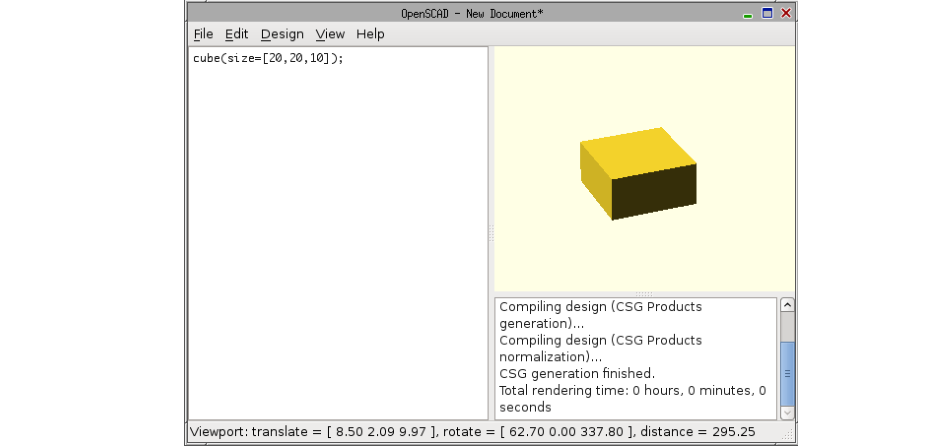
\includegraphics[width=1\textwidth]{diagrams/openSCAD.pdf}
			\caption{OpenSCAD showing a cube model compiled and rendered}
			\label{fig:openSCAD}
		\end{figure}
		
	\section{G-Code Generation (ReplicatorG \& Skeinforge)}
		
		Once an STL file has been produced, G-code for printing the model must be
		generated. ReplicatorG provides a more user-friendly front-end to the
		Skeinforge G-code generator \cite{replicatorg}. Skeinforge relies on a
		calibrated printer profile to guide its decisions. A profile was produced
		for the printer as part of the project which is compatible with ReplicatorG
		27 and Skeinforge 35 which must be copied into
		\begin{verbatim}
			replicatorg-0027/skein_engines/skeinforge-35/skeinforge_application/prefs
		\end{verbatim}
		
		Once ReplicatorG has been started, the STL file from the previous step is
		loaded using `Open' from the `File' menu (figure \ref{fig:replicatorG}).
		Once loaded, the model should be positioned centrally on the platform using
		the tools on the right of the preview. Clicking `Move' provides features to
		`Center' the model and `Put on Platform' to ensure the model is not going to
		be printed in mid-air.
		
		\begin{figure}
			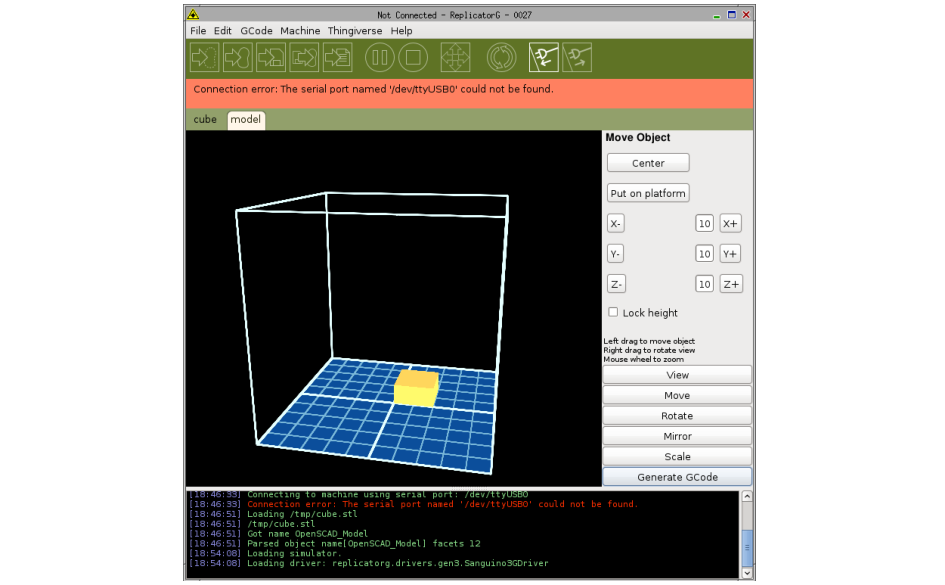
\includegraphics[width=1\textwidth]{diagrams/replicatorG.pdf}
			\caption{ReplicatorG GUI showing a cube model loaded}
			\label{fig:replicatorG}
		\end{figure}
		
		Once the model is correctly positioned, the G-code is generated using the
		`Generate GCode' button. A dialogue will prompt for a profile to be
		selected, `SF35-cupcake-ABP-raftless' should be used (figure
		\ref{fig:skeinforge}). This process can take some time for complex models
		and produces a \verb|.gcode| file containing the printer data in the same
		directory and with the same name as the STL file.
		
		\begin{figure}
			
\includegraphics[width=1\textwidth]{diagrams/skeinforge.pdf}
			\caption{Skeinforge profile selection dialogue}
			\label{fig:skeinforge}
		\end{figure}
	
	\section{Status Monitoring}
		
		To monitor the printer during a print, a utility called
		\verb|makebed_live.sh| is provided which shows heater temperatures, extruder
		position and buffer usage. It is helpful to have this open during a print to
		monitor the progress of the heating and cooling stages as well as to check
		for buffer underruns.
		
		Figure \ref{fig:makebedlive} (page \pageref{fig:makebedlive}) shows the
		utility in use during a print. Documentation is provided in appendix
		\ref{sec:makebedliveDoc}.
		
	\section{G-Code Streaming}
		
		UDP and TCP interfaces are provided for sending the G-code files generated
		by Skeinforge to the printer. Due to problems with the libraries used in the
		project, the TCP interface is currently unusable for printing purposes but
		is shown for future reference.
		
		Before any G-code is sent to the printer, the printer should me moved to its
		`home' position (figure \ref{fig:homing}). This can be done manually by hand
		or automatically by sending a G-code file containing automatic homing
		instructions\footnote{Because the Z-axis end-stops did not have a trigger
		fitted during the project, this process is currently only possible for the X
		and Y axes. See appendix \ref{sec:gcode_home_xy} for an example of such an
		automatic homing G-code file.}.
		
		\begin{figure}
			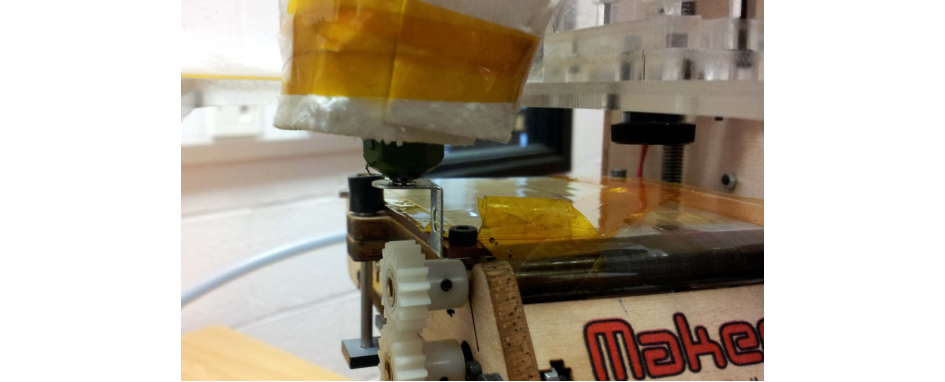
\includegraphics[width=1\textwidth]{diagrams/homing.pdf}
			\caption{Extruder placed in the homing bracket}
			\label{fig:homing}
		\end{figure}
			
		\subsection{UDP}
			
			The \verb|makebed.py| utility is used to stream a G-code file to the
			printer:
			\begin{verbatim}
				makebed.py send cube.gcode
			\end{verbatim}
			This command will block until all print data is sent to the printer.
			
			Complete documentation and safety advice for using \verb|makebed.py| to
			send files to the printer is provided in appendix \ref{sec:makebedDoc}.
			
		\subsection{TCP}
			
			The printer listens on TCP port 1818 for incoming connections. G-code sent
			to the printer via this port is executed directly and no special software
			is required. Netcat (\verb|nc|) is a standard Unix tool which can be used
			for this purpose like so:
			\begin{verbatim}
				nc -q 0 192.168.3.100 1818 < cube.gcode
			\end{verbatim}
			Where 192.168.3.100 is the IP address of the printer.
			
			Due to problems with TCP flow control in \uIP{}, this interface is
			currently not usable for printing but should become available in the
			future when the issue in \uIP{} is addressed.
	
	\section{Printing Process}
		
		The G-code generated by Skeinforge using the profile created in this project
		goes through several phases during a print. Each of these is described in
		order in the following subsections.
		
		\subsection{Warm Up \& Self-Clean}
			
			The printer first enables the platform and extruder heaters setting the
			temperatures to $120\dC$ and $225\dC$ respectively. Next, it moves the
			extruder to the heating position to the left of the platform and in front
			of the rubber cleaning peg. The printer then stays in this position until
			both heaters are up to temperature (taking around 10 to 15 minutes).
			
			Some plastic may ooze from the extruder during heating leaving an unknown
			quantity of plastic in the extruder's heating chamber. Before printing,
			the extruder must be filled with plastic and any excess wiped off against
			the cleaning peg (figure \ref{fig:selfClean}).
			
			\begin{figure}
				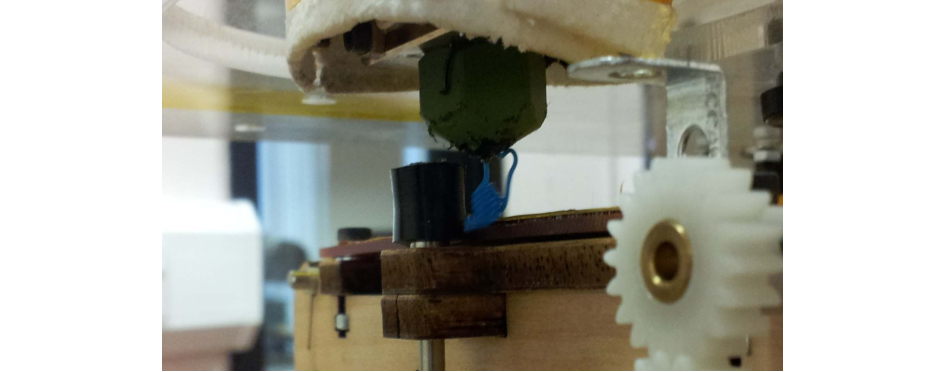
\includegraphics[width=1\textwidth]{diagrams/selfClean.pdf}
				\caption{Extruder extruding plastic during a self-clean}
				\label{fig:selfClean}
			\end{figure}
		
		\subsection{Printing The First Layer}
			
			Once everything has heated up and the extruder is free of excess plastic,
			a rectangle is drawn on the platform which surrounds the area the object
			will be printed in. This allows the operator to check that the print will
			fit on the platform and to allow manual adjustments to the height of the
			extruder to ensure that it is at the correct distance from the bed.
			
			It is critical that the distance between the extruder and platform is
			correct during the printing of the first layer. If it is too far, the
			plastic will not adhere to the platform and will not accurately produce
			the shape required. If it is too close, the plastic printed will not fit
			under the extruder causing the printed object to get caught on the
			extruder as it moves around during the print.
			
			Adjustments should be made by turning the adjustment handle on the Z-axis
			during the printing of the border. The border will be discarded after
			printing and so mistakes can be corrected while it is produced.
			
			Once the border is drawn, the extruder prints out the first layer of the
			object (figure \ref{fig:firstLayer}). This is done at a slower speed than
			other layers allowing more plastic to be deposited producing thicker
			lines. This helps the print adhere better to the platform and also
			improves the finish of the surface produced.
			
			\begin{figure}
				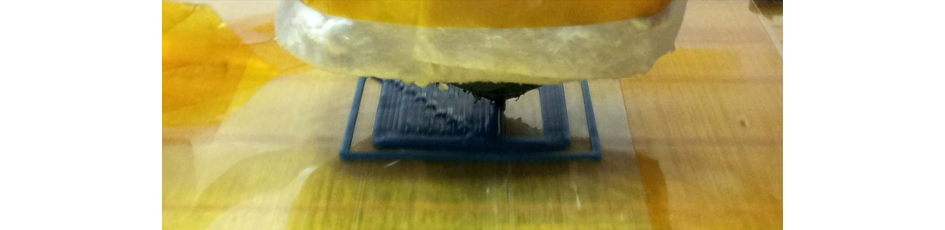
\includegraphics[width=1\textwidth]{diagrams/firstLayer.pdf}
				\caption{First layer being printed}
				\label{fig:firstLayer}
			\end{figure}
			
		\subsection{Main Printing Phase}
			
			During this phase the model is printed layer by layer. Each layer is
			usually printed first by drawing three solid shells and then filling in
			the centre. Layers near the top and bottom of the model are filled
			completely to produce a solid finish.
			
			Layers inside the model are filled with a hexagonal `fill pattern' (figure
			\ref{fig:fillPattern}). The fill pattern is not visible when the object is
			completed. It is used as it significantly reduces the time and plastic
			required to fill objects while still being strong.
			
			\begin{figure}
				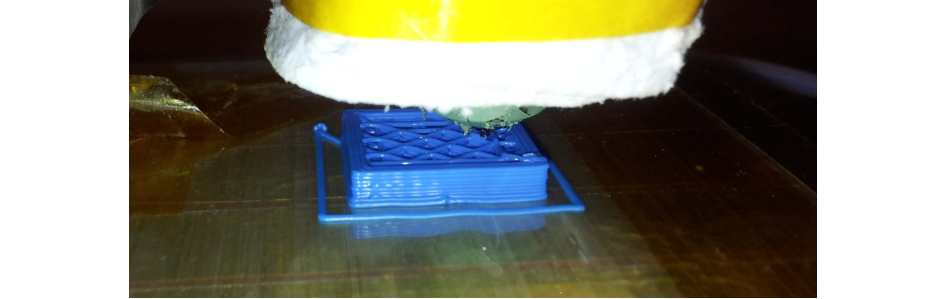
\includegraphics[width=1\textwidth]{diagrams/fillPattern.pdf}
				\caption{Fill pattern being printed}
				\label{fig:fillPattern}
			\end{figure}
			
			The cube takes around 8 minutes to print.
		
		\subsection{Cool-down, Eject and Self-Clean}
			
			Once the print completes, the platform is allowed to cool down to allow
			the object to solidify completely. This takes around 2 minutes.
			
			When the object has cooled, the platform conveyor is activated and the
			object is peeled off the platform and deposited in front of the printer.
			
			\begin{figure}
				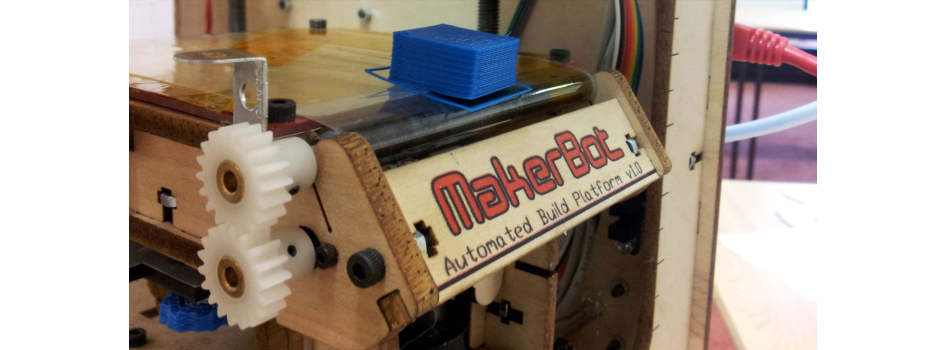
\includegraphics[width=1\textwidth]{diagrams/eject.pdf}
				\caption{Finished cuboid being ejected}
				\label{fig:eject}
			\end{figure}
			
			As plastic oozes out of the extruder after the print completes it must
			once again be cleaned using the same process as the start of the print.
			
			Finally, the printer returns to the home position and the heaters and
			power supply turned off. If another print job is started at this point,
			the extruder will still be hot but the platform, having cooled slightly,
			will need to partly reheated before the print can begin.
			
			Many prints can be run successively with no human intervention unless a
			print fails.
			
		
	\section{Final Print}
		
		Once the printer ejects the object it will still be hot and may still be
		slightly soft in some places. Care should be taken when handling the object
		until it has fully cooled.
		
		The border can be snapped off the printed cube and the process is complete.
		For more complex models, some strings of plastic left during printing
		(figure \ref{fig:stringing}) may also need to be removed using a knife.
		
		\begin{figure}
			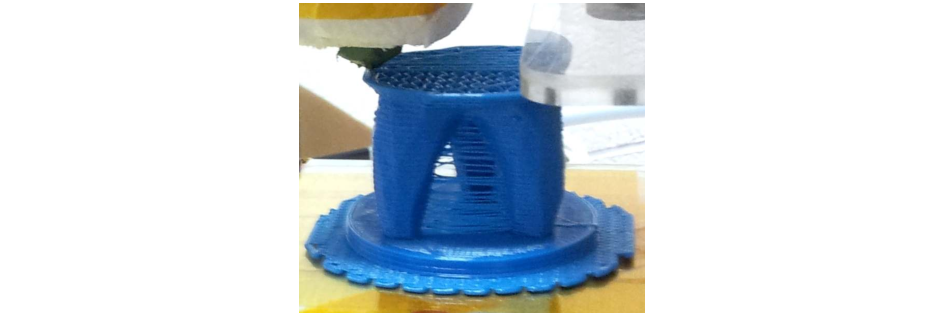
\includegraphics[width=1\textwidth]{diagrams/stringing.pdf}
			\caption{Strings of plastic left during printing requiring manual removal}
			\label{fig:stringing}
		\end{figure}

	\chapter{Example Prints}


	\chapter{Circuit Diagrams}
	
	\section{Control Electronics}
		
		\section{Pin Connection Reference}
		
		\section{Schematic}
	
	\section{Endstop Electronics}
		
		\section{Pin Connection Reference}
		
		\section{Schematic}

	\chapter{G-Code Reference}
	
	The subset of G-code interpreted by the system is described in the following
	sections.
	
	\section{Language}
		
		The G-code machine is implemented as in \S\ref{sec:gcodemachine}. The following
		subsections specify the syntax and registers of the language.
		
		\subsection{BNF}
			
			\label{sec:gcodebnf}
			
			\begin{verbatim}
				<instruction> ::= <reg-write> <new-line>
				
				<reg-write> ::= <reg-name> <number> <white-space>* <reg-write> | <comment> | ""
				<reg-name>  ::= [A-Z]
				
				<comment>            ::= <line-comment> | <block-comment>
				<line-comment>       ::= <line-comment-start> <non-newline>* <new-line> 
				<line-comment-start> ::= ";" | "/"
				<block-comment>      ::= "(" <non-close-bracket>* ")"
			\end{verbatim}
		
		\subsection{Register Types \& Behaviour}
			
			Table \ref{tab:gcoderegisters} shows the type and reset behaviour of each
			of the G-code registers.
			
			\begin{table}
				\centering
				\begin{tabular}{c l l}
					\toprule
					Register & Type & Reset at instruction start \\
					\midrule
						A & Integer & No  \\
						B & Float   & No  \\
						C & Float   & No  \\
						D & Float   & No  \\
						E & Float   & No  \\
						F & Float   & No  \\
						G & Integer & Yes \\
						H & Float   & No  \\
						I & Float   & No  \\
						J & Float   & No  \\
						K & Float   & No  \\
						L & Float   & No  \\
						M & Integer & Yes \\
						N & Float   & No  \\
						O & Float   & No  \\
						P & Integer & No  \\
						Q & Float   & No  \\
						R & Float   & No  \\
						S & Float   & No  \\
						T & Integer & No  \\
						U & Float   & No  \\
						V & Float   & No  \\
						W & Float   & No  \\
						X & Float   & No  \\
						Y & Float   & No  \\
						Z & Float   & No  \\
					\bottomrule
				\end{tabular}
				
				\caption{G-code register types and behaviours}
				\label{tab:gcoderegisters}
			\end{table}
	
	\section{Actions}
		
		\label{sec:gcodeactions}
		
		Each instruction should write a value to the `G' or `M' register. Depending
		on the value written, the printer will carry out a different action. These
		actions are specified below.
		
		\newcommand{\gcodeaction}[4]{
			\subsubsection{#1 : #2}
				#3
				
				\begin{table}[H]
					\begin{tabular}{c p{0.41\textwidth} p{0.41\textwidth}}
						\toprule
						Argument & Description & Unit \\
						\midrule
						#4
						\bottomrule
					\end{tabular}
				\end{table}
		}
		\newcommand{\gcodearg}[3]{#1 & #2 & #3 \\}
		\newcommand{\gcodenoargs}{\multicolumn{3}{c}{\emph{No arguments}}\\}
		
		\subsection{`G' Actions}
			
			\gcodeaction{G0 \& G1}{Move extruder to coordinate}{
				G1 moves the extruder through a straight line in 3D space from the
				current position to the position given in the arguments.
				
				G0 is included for compatibility reasons and does the same thing as G1.
			}{
				\gcodearg{X}{X-coordinate}{Current unit}
				\gcodearg{Y}{Y-coordinate}{Current unit}
				\gcodearg{Z}{Z-coordinate}{Current unit}
				\gcodearg{F}{Feed rate (speed) of movement}{Current unit per minute}
			}
			
			\gcodeaction{G4}{Sleep}{
				Pause the printer for a specified period.
			}{
				\gcodearg{P}{Period}{Milliseconds}
			}
			
			\gcodeaction{G20 \& G21}{Set unit}{
				Set the unit used to specify movements to inches or millimetres
				respectively.
			}{
				\gcodenoargs
			}
			
			\gcodeaction{G90 \& G91}{Set absolute/relative positioning}{
				Sets whether positions are specified absolutely or relative to the
				current position. Relative positioning is not supported by the system.
			}{
				\gcodenoargs
			}
			
			\gcodeaction{G92}{Set origin}{
				Set the current position without moving the extruder. Used to set the
				initial position of the extruder to the origin or some known homing
				location. If this instruction is not used, the current position is
				undefined and moving the extruder may have unexpected effects.
			}{
				\gcodearg{X}{X-coordinate}{Current unit}
				\gcodearg{Y}{Y-coordinate}{Current unit}
				\gcodearg{Z}{Z-coordinate}{Current unit}
			}
		
		\subsection{`M' Actions}
			
			\gcodeaction{M-2}{Home axes}{
				Custom extension to the standard G-code actions.
				
				Slowly move the specified axes until hitting the endstop. The current
				position in the X, Y and Z registers is then set to the locations of the
				end-stops (essentially calibrating the printer's position).
			}{
				\gcodearg{A}{Axis Selection}{Bit mask. Bit 1: X, Bit 2: Y, Bit 3: Z.}
			}
			
			\gcodeaction{M-1 \& M0}{Turn the PSU on/off}{
				Turns the PSU on and off respectively. Note that if the PSU is not
				powered on, many actions may block indefinitely.
				
				This action blocks until mains power is available if the
				microcontroller is being powered via USB.
				
				M-1 is a custom extension to the standard G-code actions.
			}{
				\gcodenoargs
			}
			
			\gcodeaction{M6}{Wait for heaters}{
				Block until both heaters have reached their target temperature. Contrary
				to the standard, this command will not block waiting for the heaters to
				cool down to a new target temperature.
			}{
				\gcodenoargs
			}
			
			\gcodeaction{M17 \& M18}{Power stepper motors on/off}{
				Enable or disable power to all stepper motor drivers. The steppers are
				automatically powered on when moved.
			}{
				\gcodenoargs
			}
			
			\gcodeaction{M101, M102 \& M103}{Extruder motor forward/backward/off}{
				Set the extruder motor moving forward, backward or not at all
				respectively. M102 is not supported by the system and will raise an
				error and stop the motor.
				
				The extruder should not be turned on unless it has heated up enough to
				melt the incoming filament.
			}{
				\gcodenoargs
			}
			
			\gcodeaction{M104}{Set extruder temperature}{
				Set the target temperature of the extruder. This action does not block.
				To wait for heating to complete use M6.
			}{
				\gcodearg{S}{Target temperature}{\dC}
			}
			
			\gcodeaction{M106 \& M107}{Platform conveyor on/off}{
				Turn the platform conveyor belt on or off respectively.
			}{
				\gcodenoargs
			}
			
			\gcodeaction{M108}{Set extruder speed}{
				Set the speed at which the extruder motor turns. Not supported by the
				system.
			}{
				\gcodenoargs
			}
			
			\gcodeaction{M109}{Set platform temperature}{
				Set the target temperature of the platform. This action does not block.
				To wait for heating to complete use M6.
			}{
				\gcodearg{S}{Target temperature}{\dC}
			}
	
	\section{Examples}
		
		The following examples of G-code files show how it can be used for various
		useful tasks.
		
		\subsection{Power On, Heat Up}
			
			Heats the system up to a temperature suitable for printing. Can be used to
			prepare the printer before starting a print.
			
			\begin{verbatim}
				(Turn on the PSU)
				M-1
				
				(Set the target temperature for the extruder to 225*c)
				M104 S225
				
				(Set the target temperature for the platform to 120*c)
				M109 S120
			\end{verbatim}
			
		\subsection{Power-down}
			
			Powers down all components and then the PSU. When the PSU is turned back
			on, the heaters and motors will still remain off.
			
			\begin{verbatim}
				(Turn off extruder)
				M104 S0 (Heater: set target to 0*c)
				M103    (Motor)
				
				(Turn off platform)
				M109 S0 (Heater: set target to 0*c)
				M107    (Conveyor)
				
				(Turn off stepper motors)
				M18
				
				(Power off PSU)
				M0
			\end{verbatim}
		
		\subsection{Skeinforge Print Prefix}
			
			Prefix added to all print jobs to heat up and prepare the printer before a
			print job.
			
			\begin{verbatim}
				(power on)
				M-1
				
				G21 (set units to mm)
				G90 (set positioning to absolute)
				
				(Start in parking position)
				G92 X-60 Y-45 Z10
				
				(Raise up to avoid the loop)
				G1 Z12 F100
				
				(Move to squirt position)
				G1 X-55 Y-10 F1000
				G1 Z7 F100
				
				(Heat up)
				M104 S225
				M109 S120
				M6
				
				(Extrude a bit and stop)
				M101
				G4 P5000
				M103
				G4 P6000
				
				(Wipe)
				G1 Y10 F2000
				
				(Go to origin)
				(M101)
				(G1 X0 Y0 Z0 F2400.0)
			\end{verbatim}
		
		\subsection{Skeinforge Print Postfix}
			
			Postfix added to all print jobs to cool down and eject the object after
			printing.
			
			\begin{verbatim}
				G1 X0 Y40 F3300.0 (move platform to ejection position)
				(cool down platform)
				M104 S225
				M109 S80
				M103 (Extruder off)
				G04 P100000 (wait t/1000 seconds)
				M106 (conveyor on)
				G04 P10000 (wait t/1000 seconds)
				M107 (conveyor off)
				
				(start wipe)
				(Move to squirt position)
				G1 X-55 Y-10 F1000
				G1 Z7 F100
				
				(Heat up extruder)
				M104 S225
				M6
				
				(Extrude a bit and stop)
				M101
				G4 P5000
				M103
				G4 P6000
				
				(Wipe)
				G1 Y10 F2000
				
				(Go to starting position)
				G1 Z12 F100
				G1 X-60 Y-45 F3300
				G1 Z10 F100
				
				
				(Turn off heaters)
				M104 S0 (set extruder temperature)
				M109 S0 (set heated-build-platform temperature)
				
				(power off)
				M0
			\end{verbatim}
		
		\subsection{Home X \& Y Axes}
			
			Home the X \& Y axes using the end stops. Assumes that the Z-axis is
			initially placed at the correct height to fit in the homing bracket.
			
			\begin{verbatim}
				(Power on)
				M-1
				
				(Use mm)
				G21
				
				(Set the Z axis as we're not homing that)
				G92 X0 Y0 Z10
				
				(Lift the head out of its hole)
				G1 Z15 F100
				
				(Home x[1] and y[2] at the same time[1+2 = 3])
				M-2 A3
				
				(Move to the calibration ring)
				G1 X-56 Y-44 Z15 F3300
				G1 Z10 F100
				
				(Power off)
				M0
			\end{verbatim}
			
			\label{sec:gcode_home_xy}
		
		\subsection{Circle}
			
			Plots a circle segmented into lines using the X and Y axes. Assumes the
			extruder is hovering safely above the centre of the platform before
			moving.
			
			\begin{verbatim}
				(Power on)
				M-1
				
				(Use mm)
				G21
				
				(Assume we're starting in the middle)
				G92 X0 Y0 Z0
				
				(Move to the edge of the circle)
				G1 X40.000000 Y0.000000 F330.000000
				
				(Plot the circle)
				G1 X32.360680 Y23.511410 F330.000000
				G1 X12.360680 Y38.042261 F330.000000
				G1 X-12.360680 Y38.042261 F330.000000
				G1 X-32.360680 Y23.511410 F330.000000
				G1 X-40.000000 Y0.000000 F330.000000
				G1 X-32.360680 Y-23.511410 F330.000000
				G1 X-12.360680 Y-38.042261 F330.000000
				G1 X12.360680 Y-38.042261 F330.000000
				G1 X32.360680 Y-23.511410 F330.000000
				
				(Move to the center of the circle
				G1 X0 Y0 F330.000000
				
				(Power off)
				M0
			\end{verbatim}

	\chapter{Code Documentation}
	
	\section{Configuration}
	
	\section{Utilities}
		
		\subsection{Dependencies}
		
		\subsection{Send}
		
		\subsection{Get}
		
		\subsection{makebed\_live.sh}
	
	\section{File Listing}
	
	\section{Firmware}
	
		\subsection{Dependencies}
		
		\subsection{Compilation}
			\label{sec:compilation}
	
		\subsection{Drivers}
			
			\subsubsection{Analog}
			
			\subsubsection{GPIO}
			
			\subsubsection{Watchdog}
			
		\subsection{Libraries}
			
			\subsubsection{Float Parsing}
			
			\subsubsection{Stepper}
			
			\subsubsection{Thermistor}
			
			\subsubsection{Makerbot}
			
			\subsubsection{Network}
			
			\subsubsection{PID}

	\chapter{UDP G-Code Transmission Protocol Specification}
	
	\section{Sender Packets}
	
	\section{Acknowledges}
	
	\section{Retransmission}
	
	\section{Errors}

\end{document}
